% !TEX TS-program = xelatex

% !TEX encoding = UTF-8 Unicode

\documentclass{Dissertate}

\usepackage{tikz}
\usepackage{amsmath, amssymb, amsthm}
\usepackage{graphicx}
\usepackage{microtype}
\usepackage{subcaption}
\usepackage{float}      % para [H]
\usepackage{placeins}   % para \FloatBarrier
\theoremstyle{plain}
\newtheorem{proposition}{Proposición}[chapter]
\newtheorem{Definicion}{Definición}[chapter]
\newtheorem{observacion}{Observación}[chapter]
\theoremstyle{remark}
\newtheorem{remark}{Observación}[chapter]

\usepackage{comment}
\usepackage{algorithm}
\usepackage{algpseudocode}
\begin{document}


\onehalfspacing

\setlength{\parskip}{0.5em}
\emergencystretch=2em

\frontmatter

    \setcounter{chapter}{0}
    \chapter{Diseño computacional del sistema de modelado musical}
\label{chap:design}

La tesis tiene una dimensión matemática evidente, pero también una dimensión de diseño. No basta con proponer modelos; hace falta decidir qué sistema conviene construir para analizar música simbólica bajo restricciones reales de datos, cómputo e interpretación. Este capítulo recoge esa segunda pregunta. Su función es explicitar el problema de diseño que subyace al resto del trabajo y fijar los criterios con los que se compararán soluciones clásicas y modernas.

\section{Definición del problema de diseño}

El problema de diseño consiste en construir un sistema computacional para música simbólica que permita representar secuencias discretas, modelar regularidades melódicas y armónicas, e introducir una comparación controlada entre familias de modelos con distinta complejidad. En términos musicales, interesa describir una estructura que no siempre aparece de manera explícita en la partitura; en términos computacionales, interesa decidir qué arquitectura permite hacerlo con mejor equilibrio entre ajuste, costo e inteligibilidad.

La pregunta central no es sólo qué modelo ajusta mejor, sino qué complejidad resulta defendible para el tipo de corpus y de objetivo analítico que esta tesis adopta. El problema, por tanto, no se reduce a entrenar algoritmos, sino a diseñar un sistema comparativo capaz de mostrar cuándo una solución más expresiva aporta una ventaja real y cuándo simplemente añade complejidad.

\section{Requerimientos funcionales y no funcionales}

En el plano funcional, el sistema debe aceptar entradas simbólicas en formatos estándar, convertirlas a una representación discreta común y permitir el entrenamiento y la evaluación de varios modelos sobre el mismo corpus. También debe producir salidas comparables: trayectorias inferidas, medidas de ajuste, resultados predictivos y estimaciones básicas de costo computacional.

En el plano no funcional, hay cuatro exigencias principales. La primera es la reproducibilidad: el procedimiento debe poder repetirse sobre los mismos datos y con la misma configuración experimental. La segunda es la interpretabilidad: en un problema musical no basta con predecir bien; también importa que el comportamiento del modelo conserve una lectura razonable. La tercera es la modularidad, para que el cambio de arquitectura no obligue a rehacer el pipeline completo. La cuarta es la economía computacional, entendida en relación con el alcance real de una tesis y no con condiciones de laboratorio industrial.

\section{Restricciones realistas del entorno}

Las restricciones del entorno son parte del problema y no un obstáculo exterior a él. La primera es el tamaño del corpus: en música simbólica, una tesis trabaja normalmente con colecciones pequeñas o medianas, no con volúmenes de datos propios de aplicaciones masivas. La segunda es la naturaleza de la representación: archivos como MIDI o MusicXML requieren normalización y discretización, y toda discretización supone una pérdida de información.

La tercera restricción es computacional. El diseño debe poder ejecutarse con recursos acotados y tiempos compatibles con el calendario de trabajo. La cuarta es interpretativa: en esta tesis no interesa sólo la capacidad predictiva, sino también si la estructura aprendida admite una lectura musical defendible. Esa exigencia vuelve menos atractivas las soluciones cuya expresividad depende de una opacidad excesiva.

\section{Estándares y regulaciones relevantes para el diseño}

El sistema no pertenece a un ámbito fuertemente regulado, pero sí debe respetar ciertos estándares y límites. En primer lugar, conviene trabajar con formatos simbólicos interoperables, en particular MIDI y MusicXML, para evitar que el problema dependa de codificaciones propietarias o difíciles de reproducir. En segundo lugar, el corpus y las bibliotecas empleadas están sujetos a condiciones de licenciamiento y de uso académico que no pueden ignorarse. En tercer lugar, la reproducibilidad experimental funciona aquí como un estándar metodológico: deben quedar trazables los datos usados, las transformaciones aplicadas y la configuración de cada experimento.

\section{Alternativas consideradas}

La primera alternativa es el HMM finito. Su fuerza está en la claridad de la formulación y en la interpretabilidad de los estados; su límite está en que obliga a fijar por adelantado la complejidad del espacio latente. La segunda es el HDP-HMM truncado, que conserva el marco probabilístico del HMM pero flexibiliza el número efectivo de estados. Gana en adaptabilidad, aunque al precio de una inferencia más delicada.

La tercera alternativa es un modelo basado en atención, por ejemplo un Transformer pequeño para secuencias simbólicas. Su interés radica en que puede capturar dependencias largas sin imponer explícitamente una estructura markoviana. Pero esa expresividad trae consigo un mayor costo computacional y una pérdida de legibilidad. También sería posible una solución híbrida, aunque para esta tesis esa vía complicaría la comparación más de lo que la aclararía.

\section{Arquitectura de la solución propuesta}

La solución propuesta adopta una arquitectura modular. Un primer componente se ocupa de la ingesta y normalización de archivos simbólicos. Un segundo define la representación discreta común sobre la que trabajarán todos los modelos. Un tercero implementa los modelos probabilísticos clásicos, en particular el HMM finito y el HDP-HMM truncado. Un cuarto aloja el modelo moderno basado en atención. Un quinto reúne evaluación, visualización y comparación de resultados.

La ventaja de esta estructura es simple: separa preparación de datos, modelado y análisis, y hace posible que la comparación entre arquitecturas se realice sobre una base homogénea. Así, la diferencia entre modelos puede atribuirse con mayor claridad a sus supuestos y no a cambios accidentales en el pipeline experimental.

\section{Justificación de la selección de modelos}

La elección de modelos sigue una lógica escalonada. El HMM finito ofrece una línea base clara, interpretable y barata. El HDP-HMM truncado se incorpora como extensión natural de ese marco, pues responde al problema de fijar arbitrariamente el número de estados. El modelo basado en atención aparece, en cambio, como término de contraste: no para reemplazar de antemano a los anteriores, sino para examinar si una arquitectura más expresiva compensa su mayor costo y su menor transparencia.

De este modo, la comparación no enfrenta simplemente ``lo clásico'' con ``lo moderno'', sino tres posiciones distintas ante el mismo problema: complejidad fija, complejidad flexible dentro del marco probabilístico y complejidad distribuida mediante atención.

\section{Estrategia de evaluación comparativa}

La evaluación debe realizarse sobre un mismo corpus preprocesado, con igual representación observable y con una división común entre entrenamiento, validación y prueba. De otro modo, la comparación perdería sentido. Tampoco conviene reducir el análisis a una sola métrica. Al menos deben considerarse cuatro dimensiones: ajuste estadístico, capacidad predictiva, costo computacional e interpretabilidad musical.

El interés de esta estrategia es que permite formular una conclusión de diseño y no sólo un veredicto numérico. Si un modelo basado en atención mejora apenas el ajuste, pero a cambio exige más cómputo y ofrece menos inteligibilidad, entonces esa mejora puede resultar insuficiente para justificar su adopción en este contexto.

\section{Discusión de compromisos de diseño}

El primer compromiso es el que existe entre expresividad e interpretabilidad. El segundo, entre flexibilidad estructural y estabilidad computacional. El tercero, entre ambición metodológica y alcance realista. Estos compromisos no son accidentes del trabajo: son precisamente aquello que el diseño debe ordenar.

El valor de la solución propuesta no dependerá sólo de qué modelo obtenga el mejor resultado, sino de si el sistema comparativo permite decidir con argumentos técnicos cuándo una arquitectura más compleja está justificada y cuándo no. Bajo esa luz, la parte computacional de la tesis no consiste en adoptar la técnica más reciente, sino en establecer un criterio razonable para elegir entre alternativas.

    \chapter{Preliminares}
\label{chap:introduction}

La música constituye una parte fundamental de la sociedad humana. Desde una perspectiva antropológica, puede considerarse como uno de los elementos fundacionales de múltiples culturas, al igual que las matemáticas. Ambas disciplinas comparten un impulso común: encontrar regularidad dentro de la complejidad. A partir de una motivación personal, en este trabajo se desarrollarán herramientas teóricas y marcos conceptuales que permitan explorar la intersección entre estas dos disciplinas.

El objetivo de este trabajo es caracterizar piezas musicales de manera matemática y utilizar herramientas computacionales para obtener un análisis congruente. En particular, se busca modelar la evolución melódica como un proceso estocástico en tiempo discreto y, posteriormente, incorporar estructura subyacente no directamente observable. Para ello se empleará la teoría de cadenas de Markov y, en especial, una subrama conocida como cadenas de Markov ocultas, las cuales permiten modelar sistemas dinámicos estocásticos con estados no observables directamente.

Una pieza musical puede entenderse, en primera aproximación, como una organización de eventos sonoros en el tiempo. Para convertir esa intuición en una formulación matemática se necesita fijar, al menos, tres componentes: (i) qué aspectos del sonido se consideran como información relevante, (ii) cómo se discretiza el tiempo musical, y (iii) qué tipo de dependencia se permitirá entre eventos consecutivos.

Desde un punto de vista musical, los eventos sonoros suelen describirse mediante altura (nota), duración (ritmo) y su relación con otros eventos simultáneos o consecutivos (armonía y melodía). En esta tesis se privilegia el componente melódico como objeto principal de observación: una melodía es una sucesión ordenada de notas en el tiempo. Esta elección no es meramente estética; es la que permite articular con claridad el puente hacia procesos estocásticos discretos.

El objetivo de esta parte no es desarrollar teoría musical exhaustiva, sino fijar una base mínima que justifique la representación matemática adoptada y clarifique qué se pierde y qué se conserva con las simplificaciones del modelo.

\textit{Altura (notas y clases de altura).} En el sistema occidental, las alturas musicales se organizan de manera discreta. En un instrumento como el piano, esta discretización se observa físicamente: el teclado presenta un conjunto finito de teclas por octava, y cada tecla corresponde a una frecuencia bien definida. Esta estructura permite modelar las notas como símbolos pertenecientes a un alfabeto finito. Dependiendo del nivel de abstracción, es común distinguir entre (a) \emph{notas con registro} (por ejemplo, $C_4, D_4, \dots$) y (b) \emph{clases de altura} (por ejemplo, $C, D, \dots$ identificadas módulo octava). En este trabajo se adopta un conjunto finito $S$ de símbolos musicales cuyo contenido depende de la pieza y de la representación elegida; dicho conjunto constituye el espacio de estados del modelo.

Una representación visual estándar de este conjunto discreto de alturas es el teclado del piano, en el cual las notas se disponen de manera lineal y ordenada, sugiriendo de forma natural una estructura de estados sobre la cual se definen transiciones probabilísticas.

\begin{figure}[h]
\centering
\begin{tikzpicture}[scale=1.1]

% Teclas blancas
\draw[fill=white] (0,0) rectangle (1,4);
\draw[fill=white] (1,0) rectangle (2,4);
\draw[fill=white] (2,0) rectangle (3,4);
\draw[fill=white] (3,0) rectangle (4,4);
\draw[fill=white] (4,0) rectangle (5,4);
\draw[fill=white] (5,0) rectangle (6,4);
\draw[fill=white] (6,0) rectangle (7,4);

% Teclas negras
\draw[fill=black] (0.7,2.2) rectangle (1.3,4);
\draw[fill=black] (1.7,2.2) rectangle (2.3,4);
\draw[fill=black] (3.7,2.2) rectangle (4.3,4);
\draw[fill=black] (4.7,2.2) rectangle (5.3,4);
\draw[fill=black] (5.7,2.2) rectangle (6.3,4);

% Etiquetas
\node at (0.5,-0.4) {C};
\node at (1.5,-0.4) {D};
\node at (2.5,-0.4) {E};
\node at (3.5,-0.4) {F};
\node at (4.5,-0.4) {G};
\node at (5.5,-0.4) {A};
\node at (6.5,-0.4) {B};

\end{tikzpicture}
\caption{Representación esquemática de una octava en el teclado del piano.}
\end{figure}

\textit{Ritmo y discretización temporal.} El ritmo establece la estructura temporal de la música y determina cuándo ocurren los eventos. Desde el punto de vista matemático, esto sugiere indexar la melodía mediante un parámetro temporal discreto $n\in\mathbb{N}$. En esta tesis se adopta una simplificación deliberada: se considera una malla temporal uniforme. Bajo este supuesto, cada instante de tiempo corresponde a una posición en la secuencia y el proceso musical puede representarse como una sucesión indexada $\{X_n\}_{n\ge 0}$ donde $X_n$ describe la información musical relevante en el instante $n$. Este paso implica una decisión de modelado: fenómenos como síncopas, rubato o cambios de tempo quedan fuera de la representación si no se incorporan explícitamente mediante un refinamiento temporal o variables adicionales. Aun así, la discretización uniforme constituye un punto de partida natural para el análisis computacional de melodías en notación simbólica.

\textit{Melodía, continuidad y dependencia local.} Musicalmente, una melodía no es una colección aleatoria de notas: exhibe continuidad y regularidades locales. Por ejemplo, después de una nota dada suele haber preferencia por movimientos conjuntos (intervalos pequeños) frente a saltos grandes, o bien aparecen patrones típicos (motivos) que tienden a repetirse con variaciones. Estas regularidades sugieren dependencia estocástica entre eventos consecutivos.

\textit{Armonía como estructura subyacente.} La armonía introduce relaciones simultáneas entre notas y define una organización implícita de acordes y funciones tonales. Crucialmente, dicha organización no siempre es directamente observable a partir de una sola línea melódica: una melodía puede ser compatible con varias interpretaciones armónicas, y aun así la armonía influye en qué notas son más probables en cada momento. Esta separación entre lo que se observa (notas melódicas) y lo que condiciona (contexto armónico) anticipa el paso hacia variables latentes y, por tanto, hacia cadenas de Markov ocultas.

Con estos elementos, una melodía queda representada como una sucesión de variables aleatorias
\[
(X_n)_{n\ge 0}, \qquad X_n\in S,
\]
donde $S$ es finito y corresponde a las alturas (o clases de altura) admitidas por la representación.

Una primera suposición extrema sería asumir independencia entre $X_0,X_1,\dots$, pero esto es difícil de justificar musicalmente: la elección de una nota suele depender del contexto inmediato. En el otro extremo, permitir que $X_{n+1}$ dependa de todo el historial produce un modelo muy costoso de estimar a partir de una sola pieza o de un corpus reducido. En consecuencia, emerge una hipótesis intermedia que es a la vez musicalmente interpretable y matemáticamente manejable: que el futuro dependa solamente del presente. Esta hipótesis es precisamente la propiedad markoviana.

\begin{Definicion}
Sea $(\Omega,\mathcal{F},\mathbb{P})$ un espacio de probabilidad. Una sucesión de variables aleatorias $\{X_n\}_{n \geq 0}$ con valores en un conjunto de estados $S$ se denomina \emph{cadena de Markov} si, para todo $n \geq 0$ y para cualesquiera $i_0, \ldots, i_n, j \in S$, se cumple
\[
P(X_{n+1} = j \mid X_n = i_n, \ldots, X_0 = i_0)
=
P(X_{n+1} = j \mid X_n = i_n).
\]
En forma abreviada, esta propiedad suele expresarse como
\[
P(X_{n+1}=i_{n+1}\mid X_n=i_n,\dots,X_0=i_0)=P(X_{n+1}=i_{n+1}\mid X_n=i_n).
\]
\end{Definicion}
\
En el contexto musical, el supuesto markoviano afirma que la probabilidad de la próxima nota depende únicamente de la nota actual. Esta simplificación no pretende capturar toda la gramática musical; su papel es aislar y cuantificar dependencias locales que, en muchos estilos, explican una parte relevante de la coherencia melódica.

Si el proceso se encuentra en el estado $i$, se supone que la probabilidad de transitar al estado $j$ es constante y se denota por $P_{ij}$:
\[
P(X_{n+1}=j\mid X_n=i)=P_{ij}.
\]
Estas probabilidades satisfacen
\[
P_{ij}\ge 0,\qquad \sum_{j\in S}P_{ij}=1.
\]
La matriz $\mathbf{P}=(P_{ij})_{i,j\in S}$ se denomina \emph{matriz de transición} \cite{ross2014} y encapsula la dinámica del modelo:
\[
\mathbf{P}=
    \begin{Vmatrix}
       P_{00} & P_{01} & P_{02} & \ldots \\
       P_{10} & P_{11} & P_{12} & \ldots\\
       \vdots & \vdots & \vdots & \ldots \\
       P_{i0} & P_{i1} & P_{i2} & \ldots\\
       \vdots & \vdots & \vdots & \ldots \\
    \end{Vmatrix}.
\]

En aplicaciones musicales, la matriz de transición no se especifica de manera teórica, sino que se estima empíricamente a partir de la partitura. Para cada estado $i\in S$ se contabiliza el número de veces que la nota correspondiente es seguida por cada nota $j\in S$, y se normaliza por el número total de ocurrencias de $i$. Así se obtiene un estimador de máxima verosimilitud de las probabilidades de transición, garantizando que cada renglón de $\mathbf{P}$ define una distribución de probabilidad.

Este procedimiento induce una cadena de Markov homogénea cuya estructura refleja regularidades locales de la melodía. En particular, la dependencia entre notas consecutivas queda codificada en $\mathbf{P}$, mientras que el espacio de estados captura el registro y el vocabulario melódico efectivo de la pieza. La motivación intrínseca de este modelo es caracterizar una melodía para, por un lado, entenderla con mayor profundidad y, por otro, replicarla o generar secuencias compatibles con su estilo, en el sentido estadístico local que impone la matriz de transición.
\begin{Definicion}
Un vector de probabilidad $\boldsymbol{\pi}$ se denomina \emph{distribución estacionaria} si satisface
\[
\boldsymbol{\pi}=\boldsymbol{\pi}\mathbf{P}.
\]
Si la cadena es irreducible y aperiódica, existe una única distribución estacionaria y se cumple que
\[
\lim_{n\to\infty}P(X_n=j\mid X_0=i)=\pi_j.
\]

\end{Definicion}


En el contexto musical, la distribución estacionaria describe el comportamiento estadístico global del modelo y puede interpretarse como la frecuencia relativa de aparición de cada nota en el largo plazo. En otras palabras, mientras $\mathbf{P}$ captura las dependencias locales (qué suele seguir a qué), $\boldsymbol{\pi}$ ofrece una descripción agregada del peso de cada nota dentro de la melodía, lo cual resulta útil para comparar estilos o identificar centros de gravedad melódicos.



Hasta aquí se ha considerado que la melodía observada coincide con el estado del proceso, es decir, que $X_n$ es directamente observable. Esta hipótesis es adecuada como primer modelo, pero sugiere una limitación importante: muchas regularidades musicales no se explican únicamente por la nota anterior, sino por un contexto estructural más profundo.

En particular, la armonía actúa como una organización subyacente que condiciona cuáles notas son plausibles en cada instante. Aunque una melodía sea observable, el contexto armónico que la gobierna puede no serlo de manera directa y unívoca. Desde una perspectiva probabilística, esto sugiere la existencia de variables latentes que evolucionan en el tiempo y que influyen en la distribución de las observaciones. Dicho de otra forma, la melodía puede verse como la salida observable de un sistema dinámico estocástico cuya dinámica interna no se observa completamente.

Esto conduce al problema que dará paso al siguiente capítulo: \emph{modelar la melodía como un proceso estocástico en el que la estructura armónica subyacente se representa mediante estados ocultos}. La hipótesis markoviana es razonable en este nivel latente porque las progresiones armónicas suelen exhibir dependencia local (por ejemplo, ciertas funciones tienden a seguir a otras), mientras que las notas observadas pueden interpretarse como emisiones condicionadas por dicho estado armónico. La formalización matemática de esta idea conduce a las \emph{cadenas de Markov ocultas}, que constituyen el marco principal de esta tesis y se desarrollarán a continuación.

    \chapter{Cadenas de Markov ocultas y modelado computacional}
\label{chap:hmm}

En el capítulo anterior se introdujo el uso de cadenas de Markov como un primer modelo para la caracterización matemática de melodías musicales, considerando únicamente información observable. Bajo ese enfoque, la melodía se representó como una sucesión discreta de notas y se modeló la dependencia local entre notas consecutivas mediante probabilidades de transición. Esta aproximación es útil para capturar regularidades inmediatas (por ejemplo, preferencias por movimientos conjuntos o patrones repetitivos), pero presenta limitaciones cuando se busca incorporar estructuras musicales que organizan la melodía sin estar explícitamente codificadas en la secuencia de notas.

En particular, la armonía suele actuar como una estructura subyacente que condiciona la evolución melódica: aun cuando una melodía sea completamente observable, el \emph{contexto armónico} que la hace musicalmente coherente (acordes implícitos, función tonal, tensión y resolución) no aparece necesariamente como un símbolo explícito en cada instante. Desde un punto de vista probabilístico, esto sugiere que la secuencia observable está influida por un mecanismo interno no observable directamente.

Con el objetivo de extender el marco teórico y superar estas limitaciones, en este capítulo se introduce el modelo de cadenas de Markov ocultas. Este modelo permite formalizar la coexistencia de dos niveles de descripción: un proceso estocástico oculto que captura la estructura subyacente (interpretada aquí como \emph{estado armónico} o \emph{contexto musical latente}) y un proceso observable que se genera a partir de dicho estado oculto (interpretado aquí como \emph{nota} o símbolo melódico). Además, se introducen los problemas algorítmicos fundamentales que permiten realizar inferencia eficiente, lo cual constituye el puente hacia el desarrollo computacional del proyecto.

\begin{Definicion}
Sea $(\Omega,\mathcal{F},\mathbb{P})$ un espacio de probabilidad. Una cadena de Markov oculta está definida por dos procesos estocásticos en tiempo discreto
\[
(X_n)_{n \geq 0}, \qquad (Y_n)_{n \geq 0},
\]
donde $(X_n)$ es un proceso no observable directamente u ocultos, denominado proceso oculto, y $(Y_n)$ es un proceso observable. Se fija un espacio de estados ocultos finito
\[
\mathcal{S} = \{1,2,\dots,N\},
\]
y un espacio de observaciones discreto
\[
\mathcal{V} = \{v_1,v_2,\dots,v_M\}.
\]

El proceso $(X_n)$ satisface la propiedad de Markov, es decir, para todo $n \geq 0$ y para cualesquiera $i_0,\dots,i_{n+1} \in \mathcal{S}$,
\[
P(X_{n+1} = i_{n+1} \mid X_n = i_n, \dots, X_0 = i_0)
=
P(X_{n+1} = i_{n+1} \mid X_n = i_n).
\]
Por otro lado, el proceso observable $(Y_n)$ está condicionado únicamente por el estado oculto actual. En particular, se asume que, dado $X_n$, la variable aleatoria $Y_n$ es independiente del resto del historial del proceso.
Dicho de manera más explícita: una vez conocido el estado oculto actual $X_n$, información adicional sobre estados y observaciones pasadas no modifica la distribución de $Y_n$. En símbolos, el pasado influye en $Y_n$ sólo a través del estado latente presente.
\end{Definicion}

La interpretación musical que guiará este capítulo es la siguiente. El proceso oculto $(X_n)$ representa un \emph{estado musical subyacente} que organiza la melodía; por ejemplo, puede asociarse a una función armónica, a un acorde implícito o a una región tonal que evoluciona a lo largo del tiempo. El proceso observable $(Y_n)$ representa la \emph{secuencia de notas} efectivamente registrada en la partitura (o, más generalmente, símbolos musicales observables). En este sentido, la cadena de Markov oculta formaliza la idea de que las notas son observaciones generadas a partir de un contexto armónico latente, y que dicho contexto evoluciona con dependencia local.

Una cadena de Markov oculta queda completamente determinada por el conjunto de parámetros
\[
\lambda = (\boldsymbol{\pi}, \mathbf{A}, \mathbf{B}),
\]
donde:

\begin{itemize}
    \item $\boldsymbol{\pi} = (\pi_i)_{i \in \mathcal{S}}$ es la distribución inicial del proceso oculto, con
    \[
    \pi_i = P(X_0 = i), \qquad \sum_{i=1}^N \pi_i = 1.
    \]
    \item $\mathbf{A} = (a_{ij})_{i,j \in \mathcal{S}}$ es la matriz de transición del proceso oculto, donde
    \[
    a_{ij} = P(X_{n+1} = j \mid X_n = i), \qquad \sum_{j=1}^N a_{ij} = 1.
    \]
    \item $\mathbf{B} = (b_j(v))_{j \in \mathcal{S},\, v \in \mathcal{V}}$ es la matriz de emisión, definida por
    \[
    b_j(v) = P(Y_n = v \mid X_n = j), \qquad \sum_{v \in \mathcal{V}} b_j(v) = 1.
    \]
\end{itemize}

Desde la perspectiva musical, $\boldsymbol{\pi}$ describe cuál es el contexto armónico inicial más probable; $\mathbf{A}$ describe la dinámica de cambio de contexto (por ejemplo, qué funciones armónicas tienden a seguir a cuáles); y $\mathbf{B}$ describe cómo cada contexto latente \emph{favorece} ciertas notas observables, codificando una relación estadística entre armonía y melodía.

Bajo estas hipótesis, la distribución conjunta de una trayectoria oculta $x_{0:T}$ y una secuencia observada $y_{0:T}$ factoriza como
\[
P(X_{0:T} = x_{0:T}, Y_{0:T} = y_{0:T})
=
\pi_{x_0} b_{x_0}(y_0)
\prod_{t=1}^{T} a_{x_{t-1}x_t} b_{x_t}(y_t).
\]
(añadir referencias = bloc de notas)

Esta factorización explicita la lógica generativa del modelo: primero se selecciona un estado latente inicial $X_0$ según $\boldsymbol{\pi}$; luego el estado latente evoluciona según $\mathbf{A}$; y en cada instante se genera una observación $Y_t$ según la distribución de emisión determinada por el estado oculto actual. En música, esto equivale a postular que existe un ``hilo armónico'' que evoluciona localmente y que, en cada paso, produce notas con probabilidades características del contexto en curso.

Si se considera únicamente el proceso observable $(Y_n)_{n \geq 0}$, éste no satisface en general la propiedad de Markov. Esta afirmación es relevante musicalmente: aunque el contexto armónico evolucione con memoria corta, la secuencia de notas observable puede exhibir dependencias más complejas, precisamente porque ``hereda'' la memoria del estado latente.

\begin{proposition}
El proceso observable $(Y_n)_{n\ge 0}$ de una cadena de Markov oculta no es, en general, una cadena de Markov.
\end{proposition}

\begin{proof}
Basta dar un ejemplo donde falle la propiedad de Markov. Sea $\mathcal S=\{1,2\}$ y $\mathcal V=\{0,1\}$. Defínase el proceso oculto $(X_n)$ con
\[
A=\begin{pmatrix}1&0\\0&1\end{pmatrix},
\qquad
P(X_0=1)=P(X_0=2)=\tfrac12,
\]
de modo que $X_n=X_0$ para todo $n$.

Defínase el mecanismo de emisión por
\[
P(Y_n=1\mid X_n=1)=p,\qquad P(Y_n=1\mid X_n=2)=q,
\]
con $p\neq q$ y $p,q\in(0,1)$. Entonces, condicionado en $X_0=i$, las variables $(Y_n)$ son i.i.d.\ Bernoulli con parámetro $p$ si $i=1$ y con parámetro $q$ si $i=2$.

Calculemos ahora dos probabilidades condicionales. Por la ley de la probabilidad total,
\[
P(Y_2=1,\,Y_1=1,\,Y_0=1)
=
\tfrac12\,p^3+\tfrac12\,q^3,
\qquad
P(Y_1=1,\,Y_0=1)=\tfrac12\,p^2+\tfrac12\,q^2.
\]
Por lo tanto,
\[
P(Y_2=1\mid Y_1=1,\,Y_0=1)=\frac{p^3+q^3}{p^2+q^2}.
\]
De manera similar,
\[
P(Y_2=1,\,Y_1=1)=\tfrac12\,p^2+\tfrac12\,q^2,
\qquad
P(Y_1=1)=\tfrac12\,p+\tfrac12\,q,
\]
y así
\[
P(Y_2=1\mid Y_1=1)=\frac{p^2+q^2}{p+q}.
\]

Si $(Y_n)$ fuera Markov de primer orden, debería cumplirse
\[
P(Y_2=1\mid Y_1=1,\,Y_0=1)=P(Y_2=1\mid Y_1=1).
\]
Sin embargo, para $p,q\in(0,1)$ con $p\neq q$ se tiene la desigualdad estricta
\[
\frac{p^3+q^3}{p^2+q^2}>\frac{p^2+q^2}{p+q},
\]
pues, al desarrollar la expresión,
\[
(p^3+q^3)(p+q)-(p^2+q^2)^2
=
pq\,(p-q)^2>0.
\]
Concluimos que $P(Y_2=1\mid Y_1=1,\,Y_0=1)\neq P(Y_2=1\mid Y_1=1)$, y por tanto $(Y_n)$ no satisface la propiedad de Markov de primer orden.
\end{proof}

Esta pérdida de la propiedad de Markov no constituye una deficiencia del modelo, sino una consecuencia natural de la presencia de variables latentes. En el lenguaje musical, el contexto armónico oculto actúa como una ``memoria'' adicional: incluso si sólo se observa la nota actual, la probabilidad de la siguiente nota puede depender de información previa porque el estado armónico aún no está determinado unívocamente por una sola observación.

No obstante, si se considera el proceso conjunto $(Z_n)_{n \geq 0}$ definido por
\[
Z_n = (X_n, Y_n),
\]
entonces dicho proceso sí satisface la propiedad de Markov en el espacio producto $\mathcal{S} \times \mathcal{V}$. Este resultado se establece formalmente a continuación.

\begin{proposition}
El proceso $(Z_n)_{n \geq 0} = (X_n, Y_n)$ es una cadena de Markov en el espacio de estados $\mathcal{S} \times \mathcal{V}$.
\end{proposition}

\begin{proof}
Sean $(i,v),(j,w) \in \mathcal{S} \times \mathcal{V}$ y $n \geq 0$. Por definición,
\[
\begin{aligned}
P(Z_{n+1} = (j,w) &\mid Z_n = (i,v), Z_{n-1}, \dots, Z_0) \\
&= P(X_{n+1} = j, Y_{n+1} = w \mid X_n = i, Y_n = v, \dots).
\end{aligned}
\]
Utilizando la regla del producto y las hipótesis del modelo, se obtiene
\[
\begin{aligned}
P(X_{n+1} = j, Y_{n+1} = w &\mid X_n = i, Y_n = v, \dots) \\
&= P(Y_{n+1} = w \mid X_{n+1} = j)\, P(X_{n+1} = j \mid X_n = i).
\end{aligned}
\]
La igualdad anterior se justifica por dos hechos: primero, el proceso oculto $(X_n)$ satisface la propiedad de Markov, por lo que
\[
P(X_{n+1} = j \mid X_n = i, X_{n-1}, \dots) = a_{ij};
\]
segundo, las observaciones son condicionalmente independientes del pasado dado el estado oculto actual, lo que implica
\[
P(Y_{n+1} = w \mid X_{n+1} = j, X_n, Y_n, \dots) = b_j(w).
\]
Por lo tanto,
\[
\begin{aligned}
P(Z_{n+1} = (j,w) &\mid Z_n = (i,v), Z_{n-1}, \dots, Z_0) \\
&= a_{ij}\, b_j(w),
\end{aligned}
\]
lo cual depende únicamente del estado actual $Z_n = (i,v)$. Esto prueba que $(Z_n)$ satisface la propiedad de Markov. 
\end{proof}

Este resultado pone de manifiesto que una cadena de Markov oculta puede interpretarse como una cadena de Markov ordinaria en un espacio de estados ampliado, cuya estructura particular refleja la descomposición entre la dinámica oculta y la dinámica observable. En términos musicales, al considerar simultáneamente ``contexto armónico'' y ``nota observada'' se recupera una dinámica con memoria corta, aun cuando la observación por sí sola presente dependencias más largas. \cite{cappe2005}.

En el caso particular en el que la observación determina de manera única el estado oculto, es decir, cuando existe una función determinista $f : \mathcal{V} \to \mathcal{S}$ tal que $X_n = f(Y_n)$ casi seguramente para todo $n$, el proceso observable $(Y_n)$ hereda la propiedad de Markov. Esta situación corresponde, en música, a un escenario idealizado donde cada nota identifica sin ambigüedad el contexto armónico, lo cual raramente ocurre en repertorios reales pero es útil como caso límite.

\begin{proposition}
Supóngase que existe una función determinista $f:\mathcal V\to\mathcal S$ tal que
\[
X_n = f(Y_n) \quad \text{casi seguramente para todo } n\ge 0.
\]
Entonces, el proceso observable $(Y_n)_{n\ge 0}$ es una cadena de Markov de primer orden.
\end{proposition}

\begin{proof}
Sea $v_0,\dots,v_n,v_{n+1}\in\mathcal V$. Por hipótesis, el estado oculto queda determinado de manera única por la observación, es decir,
\[
X_k = f(Y_k)\quad \text{c.s. para todo } k.
\]
En particular, conocer $Y_n=v_n$ equivale a conocer $X_n=f(v_n)$.

Consideremos la probabilidad condicional
\[
P(Y_{n+1}=v_{n+1}\mid Y_n=v_n,Y_{n-1}=v_{n-1},\dots,Y_0=v_0).
\]
Usando la ley de la probabilidad total e introduciendo el estado oculto,
\[
P(Y_{n+1}=v_{n+1}\mid Y_n=v_n,\dots)
=
P(Y_{n+1}=v_{n+1}\mid X_n=f(v_n)).
\]
Esta igualdad se debe a que, dado $Y_n=v_n$, los valores pasados $Y_{n-1},\dots,Y_0$ no aportan información adicional sobre $X_n$, pues $X_n$ queda completamente determinado por $Y_n$.

Ahora bien, por la estructura del modelo de cadena de Markov oculta,
\[
\begin{aligned}
P(Y_{n+1}=v_{n+1}\mid X_n=f(v_n))
&=
\sum_{j\in\mathcal S}
P(Y_{n+1}=v_{n+1}\mid X_{n+1}=j)\, \\
&\qquad\qquad P(X_{n+1}=j\mid X_n=f(v_n)).
\end{aligned}
\]
El lado derecho depende únicamente de $v_n$, y no del historial previo de las observaciones. Por lo tanto,
\[
\begin{aligned}
P(Y_{n+1}=v_{n+1} &\mid Y_n=v_n,Y_{n-1},\dots,Y_0) \\
&= P(Y_{n+1}=v_{n+1}\mid Y_n=v_n),
\end{aligned}
\]
lo que prueba que $(Y_n)$ satisface la propiedad de Markov de primer orden.
\end{proof}

\begin{observacion}
La igualdad $X_n = f(Y_n)$ debe entenderse en el sentido de igualdad entre variables aleatorias, es decir, casi seguramente. Dado que $X_n$ y $Y_n$ son funciones definidas sobre un espacio de probabilidad común, exigir igualdad punto a punto no es necesario ni natural en este contexto. En efecto, dos variables aleatorias que difieren únicamente en un conjunto de probabilidad nula inducen las mismas probabilidades condicionales y, por tanto, son indistinguibles desde el punto de vista del análisis estocástico. En consecuencia, la hipótesis $X_n = f(Y_n)$ c.s.\ es suficiente para garantizar que la observación determina completamente el estado oculto a nivel probabilístico. \cite{cappe2005}
\end{observacion}

\section{Problemas fundamentales de Markov oculto}

Una vez fijado el modelo, las preguntas relevantes no son únicamente ``qué es'' una cadena de Markov oculta, sino qué se puede \emph{inferir} a partir de ella. En el contexto musical, esto se traduce en dos tareas centrales: cuantificar qué tan compatible es una secuencia de notas con un modelo (por ejemplo, con un estilo armónico-melódico aprendido) y reconstruir el contexto latente más probable que pudo haber generado la melodía observada. Ambas tareas se formalizan en los problemas clásicos de evaluación y decodificación.

Dado un modelo $\lambda$ y una secuencia observada $y_{0:T}$, se consideran tres problemas clásicos en la teoría de cadenas de Markov ocultas: evaluación, aprendizaje y decodificación. Para el presente trabajo los dos problemas más relevante son el de evaluación y decodificación. Aprendizaje fue un paradigma durante muchos años para modelos de inteligencia artificial pero estos han sido sobrepasados por tecnologías mas modernas, a continuación se explica en detalle estos problemas.

\subsection{Evaluación}

Sea un modelo
\[
\lambda = (\boldsymbol{\pi}, \mathbf{A}, \mathbf{B})
\]
y una secuencia de observaciones
\[
y_{1:T} = (y_1, y_2, \dots, y_T).
\]
El problema de evaluación consiste en determinar la probabilidad
\[
P(y_{1:T} \mid \lambda).
\]
En música, esta cantidad puede interpretarse como un puntaje de verosimilitud: mide qué tan plausible es la secuencia de notas observada bajo el modelo armónico-latente propuesto.

Aunque esta probabilidad puede calcularse directamente mediante argumentos probabilísticos clásicos, dicho enfoque requiere considerar todas las posibles trayectorias de estados ocultos, lo cual involucra $N^T$ operaciones y resulta computacionalmente inviable incluso para valores moderados de $T$. Este obstáculo es especialmente relevante en análisis musical, donde una melodía real puede tener cientos o miles de instantes discretos.

Para resolver este problema de manera eficiente se introduce una variable auxiliar $\alpha_t(i)$, denominada \emph{variable hacia adelante} (\emph{forward variable}), definida como
\[
\alpha_t(i) = P(y_1, y_2, \dots, y_t, X_t = i \mid \lambda).
\]
Estas variables satisfacen la siguiente relación recursiva:
\[
\alpha_{t+1}(j) = b_j(y_{t+1}) \sum_{i=1}^N \alpha_t(i)\, a_{ij},
\qquad 1 \le j \le N,\; 1 \le t \le T-1,
\]
con condiciones iniciales
\[
\alpha_1(j) = \pi_j\, b_j(y_1), \qquad 1 \le j \le N.
\]
La probabilidad total de la secuencia observada queda entonces dada por
\[
P(y_{1:T} \mid \lambda) = \sum_{i=1}^N \alpha_T(i).
\]
La complejidad computacional de este algoritmo es del orden $O(N^2T)$, lo cual representa una mejora exponencial con respecto al cálculo directo.

Desde el punto de vista interpretativo, $\alpha_t(i)$ cuantifica la probabilidad de que, tras escuchar (u observar) los primeros $t$ símbolos de la melodía, el estado armónico latente en el instante $t$ sea $i$. Así, el algoritmo \emph{forward} puede verse como un mecanismo de propagación de creencias sobre el contexto armónico conforme avanza la melodía.

\subsection{Decodificación }

El problema de decodificación en una cadena de Markov oculta consiste en determinar, dada una secuencia observada, una trayectoria de estados ocultos que maximice la probabilidad posterior. En el caso estándar, este problema se formula como la búsqueda de la trayectoria que maximiza la probabilidad conjunta con la secuencia observada.

En música, esta tarea se interpreta como la reconstrucción de la secuencia de contextos latentes más probable (por ejemplo, la progresión armónica implícita) que pudo haber generado las notas observadas, bajo el modelo $\lambda$. El algoritmo de Viterbi resuelve este problema de manera eficiente mediante programación dinámica. En lugar de enumerar todas las posibles trayectorias ocultas, cuya cantidad crece exponencialmente con la longitud de la secuencia, el algoritmo explota la estructura markoviana del modelo para construir soluciones óptimas parciales que se combinan recursivamente.

Sea $y_{0:T}$ una secuencia observada. Se define
\[
\delta_t(j) = \max_{x_{0:t-1}} P(X_{0:t-1} = x_{0:t-1}, X_t = j, Y_{0:t} = y_{0:t}),
\]
con condiciones iniciales
\[
\delta_0(j) = \pi_j b_j(y_0),
\]
y la recurrencia
\[
\delta_t(j) = b_j(y_t) \max_{i \in \mathcal{S}} \delta_{t-1}(i) a_{ij}.
\]
La trayectoria óptima se obtiene mediante un procedimiento de retroceso a partir de
\[
\hat{x}_T = \arg\max_{j \in \mathcal{S}} \delta_T(j).
\]
Las ecuaciones anteriores describen la lógica del método; el pseudocódigo siguiente resume su implementación paso a paso.

\begin{algorithm}[H]
\caption{Algoritmo de Viterbi}
\label{alg:viterbi}
\begin{algorithmic}[1]
\Require Observaciones $O=(o_1,\dots,o_T)$, estados $S=\{1,\dots,N\}$,
probabilidades iniciales $\boldsymbol{\pi}$, matriz de transición $A=(a_{ij})$,
probabilidades de emisión $B=(b_j)$
\Ensure Secuencia de estados más probable $X^*=(x_1^*,\dots,x_T^*)$

\Statex
\State \textbf{Inicialización}
\For{$j = 1$ \textbf{to} $N$}
    \State $\delta_1(j) \gets \pi_j\, b_j(o_1)$
    \State $\psi_1(j) \gets 0$
\EndFor

\Statex
\State \textbf{Recursión}
\For{$t = 2$ \textbf{to} $T$}
    \For{$j = 1$ \textbf{to} $N$}
        \State $\displaystyle 
        \delta_t(j) \gets 
        \max_{1 \le i \le N} \bigl[ \delta_{t-1}(i)\, a_{ij} \bigr]\; b_j(o_t)$
        \State $\displaystyle 
        \psi_t(j) \gets 
        \arg\max_{1 \le i \le N} \bigl[ \delta_{t-1}(i)\, a_{ij} \bigr]$
    \EndFor
\EndFor

\Statex
\State \textbf{Terminación}
\State $\displaystyle P^* \gets \max_{1 \le j \le N} \delta_T(j)$
\State $\displaystyle x_T^* \gets \arg\max_{1 \le j \le N} \delta_T(j)$

\Statex
\State \textbf{Retropropagación}
\For{$t = T-1, T-2, \dots, 1$}
    \State $x_t^* \gets \psi_{t+1}(x_{t+1}^*)$
\EndFor

\Statex
\Return $X^* = (x_1^*,\dots,x_T^*)$
\end{algorithmic}
\end{algorithm}
\cite{bouguila2020}

En términos musicales, el resultado de Viterbi entrega la ``explicación latente'' más probable de la melodía: una trayectoria $X^*$ que puede interpretarse como la secuencia de contextos armónicos que mejor justifica las notas observadas bajo el modelo. Esto es particularmente valioso cuando se desea comparar interpretaciones armónicas implícitas o estudiar cómo cambia la estructura subyacente a lo largo de una pieza.

El modelo oculto encuentra una limitación importante: puede ocurrir que algunos estados latentes no sean efectivamente visitados o inferidos a partir de los datos disponibles. Dado que los estados ocultos suelen representar clases de contexto (por ejemplo, funciones o configuraciones armónicas), es posible que ciertas configuraciones nunca aparezcan en una pieza o en un corpus pequeño, lo cual induce probabilidades de transición o emisión nulas en una estimación puramente frecuentista. Este fenómeno no sólo es computacional (porque puede bloquear trayectorias en Viterbi), sino también interpretativo (porque restringe artificialmente el espacio de explicaciones armónicas). A continuación se presenta un ejemplo de este caso.

Se realizó una prueba con la pieza \emph{Preludio en Do Mayor} de J.\,S. Bach (1685--1750) utilizando los siguientes parámetros. La matriz de transición $\mathbf{A}=(A_{ij})$ se define sobre los \emph{estados ocultos} (interpretados aquí como acordes, o triadas de notas). En este tipo de estudios es común imponer una estructura homogénea de la forma
\begin{equation}
A_{ii} \;=\; \frac{\alpha}{\alpha+(N-1)\beta},
\qquad
A_{ij} \;=\; \frac{\beta}{\alpha+(N-1)\beta}\quad (i\neq j),
\label{eq:transicion_alpha_beta}
\end{equation}
donde $N=\lvert\mathcal{S}\rvert$ es el número de estados ocultos. Aquí $\alpha$ controla la permanencia en el mismo estado, mientras que $\beta$ regula la probabilidad de transición hacia estados distintos. Con esta parametrización, la probabilidad de \emph{cambiar} de acorde en un paso es baja, mientras que la probabilidad de \emph{permanecer} en el mismo acorde es alta.

En nuestro caso fijamos $\alpha=210$ y $\beta=1$, y tomamos una distribución inicial uniforme,
\[
\pi_i=\frac{1}{N},\qquad i=1,\dots,N.
\]
Esta elección significa que, al inicio, ningún acorde se privilegia \emph{a priori} sobre otro: antes de observar la secuencia, todos los estados ocultos se consideran igualmente plausibles.
Por ejemplo, si $N=24$, entonces
\[
A_{ii}=\frac{210}{210+23}\approx 0.901,
\qquad
\sum_{j\neq i}A_{ij}=\frac{23}{210+23}\approx 0.099,
\]
es decir, la probabilidad de quedarse en el mismo acorde es aproximadamente $0.9$ y la de moverse a un acorde distinto es aproximadamente $0.1$.

Se analizó esta pieza debido a que el conteo manual de las transiciones armónicas resulta relativamente accesible. Esto permite construir una matriz de transición “real” basada directamente en la partitura y utilizarla como referencia para evaluar el desempeño del modelo oculto. De esta manera, se dispone de un criterio empírico claro para comparar la estructura armónica inferida algorítmicamente con la estructura efectivamente observada en la obra.

El procedimiento seguido fue el siguiente. Primero, se identificó manualmente la sucesión de acordes presentes en la pieza y se construyó la matriz de transiciones empírica mediante conteo directo y normalización por renglones. Posteriormente, utilizando el modelo de cadena de Markov oculta con los parámetros previamente especificados, se aplicó el algoritmo de Viterbi para obtener la trayectoria latente más probable de estados armónicos. A partir de esta trayectoria inferida, se reconstruyó la matriz de transiciones correspondiente y se comparó con la matriz real.

\bigskip

\begin{figure}[H]
    \centering
    \begin{subfigure}{0.9\textwidth}
        \centering
        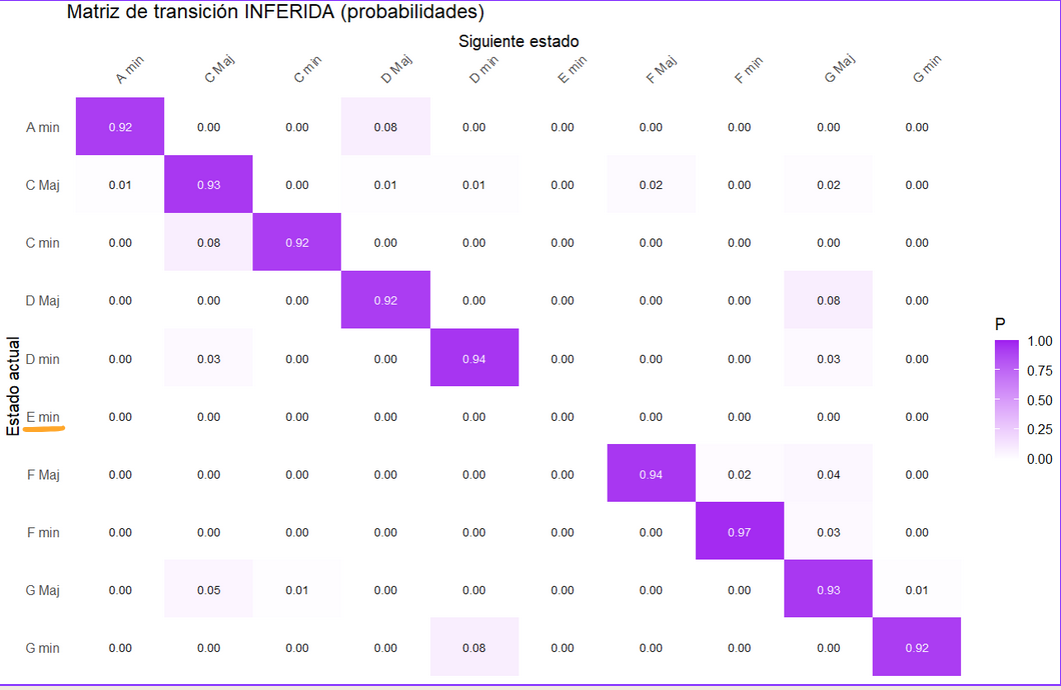
\includegraphics[width=\linewidth]{figures/Inferida.png}
        \caption{Matriz inferida mediante Viterbi}
        \label{fig:matriz_inferida}
    \end{subfigure}
    
    \medskip
    \begin{subfigure}{0.9\textwidth}
        \centering
        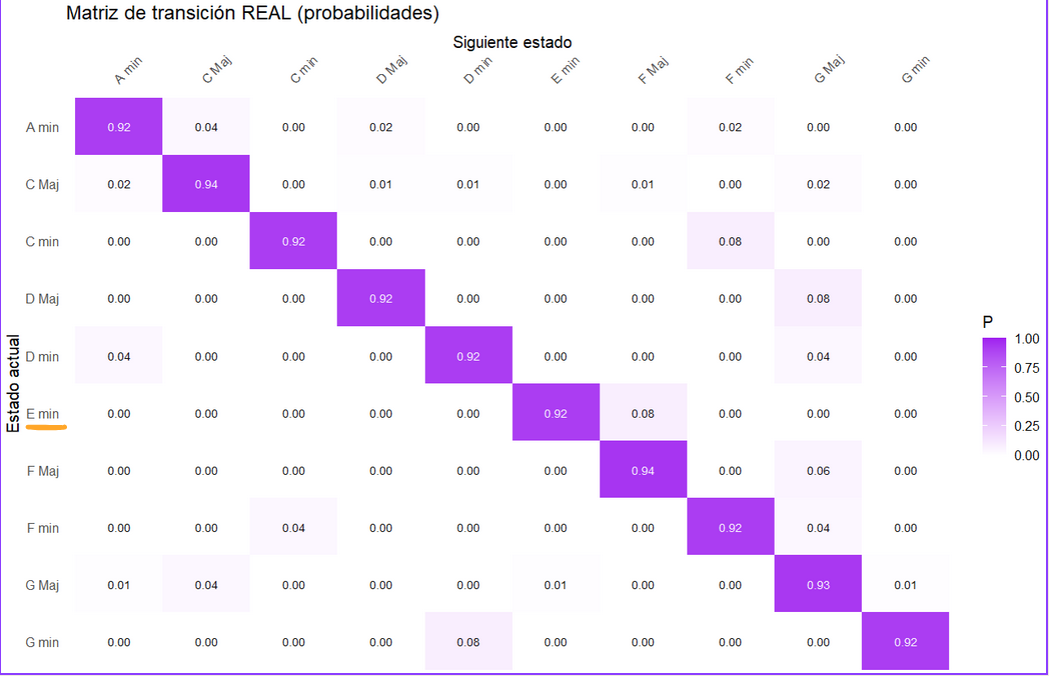
\includegraphics[width=\linewidth]{figures/real.png}
        \caption{Matriz real de transiciones}
        \label{fig:matriz_real}
    \end{subfigure}
    \caption{Comparación entre la matriz de transiciones armónicas inferida por el modelo oculto y la matriz obtenida mediante conteo directo de la partitura. En ambas, los tonos más oscuros indican probabilidades de transición más altas.}
    \label{fig:comparacion_matrices}
\end{figure}

\newpage

La comparación entre ambas matrices muestra con claridad tanto el alcance como la limitación del método. El modelo no observa acordes de manera directa, sino únicamente notas emitidas por estados latentes; por ello, la reconstrucción armónica que obtiene es necesariamente parcial. Aun así, las probabilidades dominantes, en particular las entradas diagonales asociadas a permanencia y varias de las transiciones estructuralmente frecuentes, coinciden cualitativamente con la matriz obtenida por conteo directo. Esto sugiere que la hipótesis de una dinámica markoviana latente resulta razonable para esta pieza. En total, la obra presenta $30$ cambios de acorde; el algoritmo identifica $27$ de ellos, es decir, el $90\%$. Entre esas $27$ transiciones detectadas, $22$ coinciden con la referencia manual, lo que equivale aproximadamente al $82\%$.

\bigskip    


\FloatBarrier
\begin{figure}[H]
    \centering
    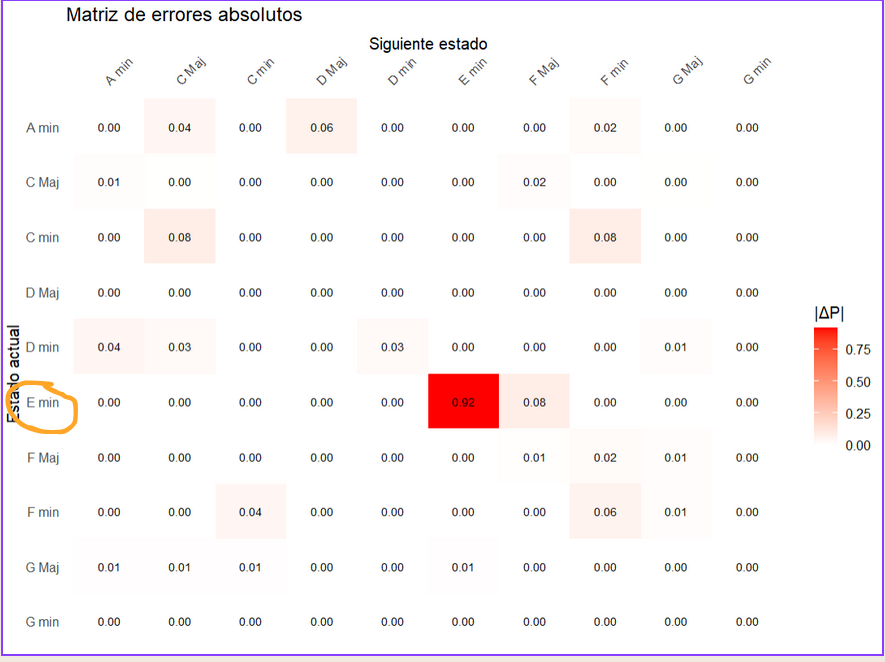
\includegraphics[width=0.82\linewidth]{figures/Error.png}
    \caption{Matriz de error de la estimación.}
    \label{fig:MatrizErr}
\end{figure}
\FloatBarrier

Esta limitación fundamental pone en evidencia la necesidad de expandir el alcance del modelo tradicional. Con el propósito de superar estas deficiencias estructurales, se ha propuesto diversas extensiones orientadas a dotar de mayor capacidad expresiva a las cadenas de Markov ocultas. 

En particular, una de estas alternativas consiste en las cadenas de Markov ocultas infinitas. Este modelo relaja la restricción de operar sobre un espacio de estados finito, asumiendo, en su lugar, una cardinalidad infinita para el conjunto de estados latentes. La premisa subyacente es que dicha formulación proporciona una representación armónica de mayor fidelidad, en tanto permite estimar y modelar la diversidad inherente de configuraciones musicales (como los acordes) con mayor precisión.

Conviene subrayar que el paso hacia este nuevo modelo no abandona la lógica desarrollada en el presente capítulo. Hasta aquí, la pregunta central ha sido: dado un HMM ya especificado, ¿cómo evaluar una secuencia observada y cómo reconstruir su trayectoria latente más probable? El capítulo siguiente conserva exactamente esa intuición musical, pero desplaza la dificultad a un nivel anterior: antes de inferir, hay que decidir cuántos estados armónicos necesita realmente el modelo para describir una pieza o un corpus sin colapsar distinciones relevantes ni inflar artificialmente el vocabulario.

Dicho de otro modo, el problema ya no será solamente \emph{cómo inferir} estados ocultos, sino también \emph{cuánta complejidad latente conviene permitir}. Esa pregunta conduce de manera natural al marco no paramétrico bayesiano: en lugar de fijar de antemano un inventario cerrado de contextos armónicos, se busca que la complejidad efectiva del modelo emerja de los datos observados.

    \chapter{Cadenas de Markov ocultas infinitas} 
\label{sec:proyecto}

En el capítulo anterior se introdujo el modelo de cadenas de Markov ocultas como una formulación probabilística para describir la coexistencia de un proceso latente y una secuencia observable. En el contexto musical, esta idea permitió interpretar las notas observadas como emisiones generadas por un mecanismo interno no directamente visible, el cual puede asociarse a una estructura armónica, a una región tonal o, más generalmente, a un contexto musical subyacente.

Tal descripción resulta adecuada siempre que se acepte que la dinámica latente puede resumirse en un conjunto finito de estados. El problema de este capítulo aparece precisamente cuando esa hipótesis comienza a quedarse corta para describir un vocabulario armónico más flexible.

Así, el cambio respecto del capítulo anterior no consiste en introducir un objeto musical distinto, sino en reformular una decisión de modelado que hasta ahora permanecía fija. En el HMM finito, una vez elegido el número de estados, los algoritmos de evaluación e inferencia pueden aplicarse de manera directa; pero en aplicaciones musicales esa elección rara vez es inocua. Un vocabulario demasiado pequeño fusiona contextos armónicos con funciones distintas, mientras que uno demasiado grande fragmenta regularidades que sería preferible mantener unificadas.

La pregunta guía del capítulo puede formularse así: si la idea latente-observable del HMM sigue siendo musicalmente útil, pero el número de estados deja de ser evidente, ¿cómo permitir que el propio modelo ajuste su complejidad al repertorio analizado? Para responderla, primero se fija una línea base finita y después se introduce la extensión no paramétrica que relaja esa decisión.

En una formulación armónica concreta, el HMM clásico exige fijar primero un conjunto finito $S$ de acordes permitidos y, una vez enumerado, identificar el espacio de estados ocultos con
\[
\mathcal{S}=\{1,2,\dots,N\},
\qquad N=\lvert S\rvert.
\]
La elección de $S$ determina simultáneamente la dimensión de la distribución inicial $\boldsymbol{\pi}$, de la matriz de transición $\mathbf{A}$ y de la familia de distribuciones de emisión $\mathbf{B}$. Para mantener comparabilidad e interpretabilidad, se adopta un vocabulario armónico finito construido como pares de la forma
\[
(\text{fundamental},\text{plantilla armónica}).
\]
El primer componente recoge la clase de altura y el segundo la sonoridad admitida.

Sea
\[
\mathcal{R}
=
\{C,C^\sharp,D,E^\flat,E,F,F^\sharp,G,A^\flat,A,B^\flat,B\}
\]
el conjunto de clases de altura fundamentales. Sea además
\[
\mathcal{Q}=
\left\{
\begin{array}{@{}l@{}}
\mathrm{Maj},\mathrm{min},\mathrm{dim},\mathrm{aug},\\
\mathrm{Maj7},7,\mathrm{m7},\mathrm{m(Maj7)},\varnothing 7,\mathrm{dim7},\\
6,\mathrm{m6},\mathrm{add9},\mathrm{madd9},6/9,\\
\mathrm{sus2},\mathrm{sus4},7\mathrm{sus4},\\
\mathrm{Maj9},9,\mathrm{m9}
\end{array}
\right\}
\]
la familia de plantillas armónicas admitidas. Con ello se obtiene un repertorio suficientemente rico para distinguir triadas, séptimas, suspensiones y extensiones frecuentes sin volver opaco el espacio latente.

Se define entonces
\[
S=\mathcal{R}\times\mathcal{Q}.
\]
En consecuencia,
\[
\lvert S\rvert = 12\times 21 = 252.
\]
Este tamaño sigue siendo manejable para un HMM finito con observaciones discretas y evita colapsar sonoridades distintas sobre una misma triada elemental. Sin embargo, la decisión sigue siendo exógena: si $N$ es demasiado pequeño, el modelo fusiona funciones distintas; si es demasiado grande, fragmenta regularidades y dispersa masa de probabilidad. El problema central, entonces, no es sólo enriquecer el vocabulario armónico, sino permitir que la complejidad efectiva del espacio latente dependa de los datos y no de una elección previa.

\section{Modelos bayesianos no paramétricos para secuencias musicales}

La situación anterior conduce al marco de los modelos bayesianos no paramétricos. Aquí \emph{no paramétrico} no significa ausencia de parámetros, sino ausencia de una cota fijada de antemano para la complejidad estructural del modelo. La herramienta central es el proceso de Dirichlet, que permite definir distribuciones a priori sobre medidas de probabilidad discretas \cite{ferguson1973,sethuraman1994}. Una discusión más amplia de esta construcción y de su versión jerárquica se deja al Apéndice A; en el cuerpo principal basta retener que el objetivo es reemplazar la elección exógena de $N$ por un mecanismo probabilístico capaz de reutilizar estados ya activados y, al mismo tiempo, introducir nuevos cuando la secuencia lo exige.

La primera extensión natural del HMM clásico consiste entonces en reemplazar el espacio finito de estados ocultos por un conjunto numerable infinito, que para fijar ideas se identifica con
\[
\mathcal{S}=\mathbb{N}.
\]
La hipótesis markoviana no se modifica: el futuro del proceso oculto depende únicamente del estado oculto presente, y cada observación depende solamente del estado latente actual. Lo que cambia es la cardinalidad del conjunto sobre el cual se definen las transiciones.

\begin{Definicion}
Una \emph{cadena de Markov oculta infinita} está determinada por dos procesos estocásticos en tiempo discreto
\[
(X_n)_{n\geq 0}, \qquad (Y_n)_{n\geq 0},
\]
donde $(X_n)$ toma valores en $\mathbb{N}$ y $(Y_n)$ toma valores en un espacio de observaciones $\mathcal{V}$. Se fija una distribución inicial
\[
\boldsymbol{\pi}=(\pi_i)_{i\geq 1},
\]
una matriz de transición infinita
\[
\mathbf{A}=(a_{ij})_{i,j\geq 1},
\]
y una familia de distribuciones de emisión
\[
\mathbf{B}=(b_j)_{j\geq 1},
\]
de modo que, para todo $i,j\geq 1$ y todo $v\in\mathcal{V}$,
\[
P(X_0=i\mid \boldsymbol{\pi})=\pi_i,
\]
\[
P(X_{n+1}=j\mid X_n=i,\mathbf{A})=a_{ij},
\qquad
P(Y_n=v\mid X_n=j,\mathbf{B})=b_j(v),
\]
con
\[
\sum_{i=1}^{\infty}\pi_i=1,
\qquad
\sum_{j=1}^{\infty}a_{ij}=1,
\qquad
\sum_{v\in\mathcal{V}}b_j(v)=1.
\]
\end{Definicion}

La definición anterior extiende literalmente la formulación del HMM al caso de un espacio de estados ocultos numerable. La estructura markoviana y la factorización de la ley conjunta se conservan; lo que cambia es la forma de controlar la complejidad del espacio latente.

La dificultad principal consiste en coordinar coherentemente los renglones de una matriz de transición infinita. Para ello se introduce una medida global que actúa como soporte compartido de las distribuciones de transición. Esta construcción conduce al proceso de Dirichlet jerárquico y, en el contexto de cadenas de Markov ocultas, al \emph{HDP-HMM} (\emph{Hierarchical Dirichlet Process Hidden Markov Model}), que proporciona una realización concreta del \emph{Infinite Hidden Markov Model (iHMM)} \cite{beal2002,teh2006}.

En esta formulación se introduce una medida discreta aleatoria global
\[
\beta=\sum_{k=1}^{\infty}\beta_k\delta_k,
\]
donde
\[
\beta_k=v_k\prod_{\ell=1}^{k-1}(1-v_{\ell}),
\qquad
v_k \overset{i.i.d.}{\sim}\mathrm{Beta}(1,\gamma),
\qquad k\geq 1,
\]
y se supone que
\[
\boldsymbol{\pi}\mid \beta \sim DP(\alpha_0,\beta),
\qquad
A_i\mid \beta \sim DP(\alpha,\beta), \qquad i\geq 1,
\]
donde $A_i$ denota el renglón $i$-ésimo de $\mathbf{A}$.
\[
\mathbb{E}[a_{ij}\mid\beta]=\beta_j.
\]
La medida global $\beta$ asigna pesos a una familia numerable de estados potenciales y acopla todas las distribuciones de transición al imponerles un soporte común. En términos musicales, esto permite reutilizar contextos latentes ya presentes sin impedir que aparezcan otros cuando la evidencia secuencial lo justifica.

Cuando el espacio observable $\mathcal{V}$ es finito, como ocurre al modelar notas, clases de altura, intervalos o símbolos rítmicos discretizados, la familia de emisiones $\mathbf{B}$ puede mantenerse dentro de una parametrización finita ordinaria. En muchas aplicaciones musicales esta decisión es suficiente, porque la principal fuente de incertidumbre no suele residir en el alfabeto observable, sino en cuántos contextos latentes hacen falta para organizarlo en el tiempo.

La infinitud del espacio de estados no implica que una pieza finita requiera infinitos contextos latentes, sino que el modelo deja abierta esa complejidad y la delega a la inferencia. Ésta es la diferencia decisiva frente al HMM clásico: en lugar de fijar primero el número de estados y luego estimar transiciones y emisiones, el iHMM permite que la estructura latente emerja del comportamiento observado. Para el análisis musical, esto significa que distinciones armónicas, melódicas o formales sólo se separan cuando los datos ofrecen evidencia suficiente para hacerlo.



\section{Aproximación truncada y formulación computacional}

La formulación infinita descrita en la sección anterior tiene valor conceptual, pero su uso directo en inferencia complica la implementación porque la programación dinámica debe operar sobre un conjunto no acotado de estados potenciales. Por ello, en la práctica se emplea una aproximación truncada que conserva la estructura jerárquica del HDP-HMM y la proyecta sobre un simplex finito de dimensión $K$ \cite{ishwaran2001,fox2011,vangael2008}.

\begin{Definicion}
Fijado un entero $K\geq 2$, un \emph{HDP-HMM truncado} con espacio observable discreto $\mathcal{V}=\{1,\dots,V\}$ queda determinado por las variables aleatorias
\[
v_k\sim \mathrm{Beta}(1,\gamma), \qquad k=1,\dots,K-1,
\]
\[
\beta_k=v_k\prod_{\ell=1}^{k-1}(1-v_{\ell}), \qquad k=1,\dots,K-1,
\]
\[
\beta_K=\prod_{\ell=1}^{K-1}(1-v_{\ell}),
\]
por el vector global $\beta=(\beta_1,\dots,\beta_K)$ y por las distribuciones condicionadas
\[
\boldsymbol{\pi}\mid \beta \sim \mathrm{Dir}(\alpha_0\beta_1,\dots,\alpha_0\beta_K),
\]
\[
A_i\mid \beta \sim \mathrm{Dir}(\alpha\beta+\kappa e_i), \qquad i=1,\dots,K,
\]
\[
\phi_i\sim \mathrm{Dir}\left(\frac{\eta}{V},\dots,\frac{\eta}{V}\right), \qquad i=1,\dots,K,
\]
donde $e_i$ denota el $i$-ésimo vector canónico de $\mathbb{R}^K$. La cadena latente y las observaciones satisfacen entonces
\[
X_1\mid \boldsymbol{\pi}\sim \mathrm{Cat}(\boldsymbol{\pi}),
\qquad
X_t\mid X_{t-1}=i,\mathbf{A}\sim \mathrm{Cat}(A_i),
\]
\[
Y_t\mid X_t=i,\phi_i\sim \mathrm{Cat}(\phi_i), \qquad t\geq 1.
\]
\end{Definicion}

La escritura anterior conserva la lógica del modelo infinito: $\beta$ organiza el soporte compartido, $\alpha_0$ regula la distribución inicial y $\alpha$ controla cuánto puede apartarse cada renglón de la estructura global. En la práctica, lo importante es escoger un $K$ suficientemente amplio para que funcione como cota técnica y no como restricción activa. Una vez fijado, las transiciones y emisiones pueden manejarse como matrices finitas y la trayectoria latente puede inferirse con programación dinámica estándar, con costo dominante del orden de $O(TK^2)$.

En esta tesis, el modelo truncado se especializa al caso de observaciones categóricas de clase de altura. El iHMM conserva así su papel como referencia conceptual, mientras que el HDP-HMM truncado se vuelve la realización operativa con la que se efectúan los experimentos reproducibles y la comparación con el HMM finito.

\section{De una obra al corpus}

Antes de pasar a resúmenes agregados conviene fijar un caso singular que obligue al modelo a mostrar su conducta en condiciones exigentes. En lugar de empezar por promedios, se toma como obra ancla el tercer movimiento de la Sonata no.\ 14 de Beethoven, una pieza extensa dentro del corpus extendido, con $4133$ notas y $201$ compases. La elección no pretende canonizar una sola obra, sino introducir una situación en la que el HMM finito tiende a fragmentar en exceso el espacio latente y donde, por tanto, la promesa del modelo no paramétrico puede evaluarse de forma visible.

La Tabla~\ref{tab:single-anchor} resume el contraste cuantitativo. El HMM finito activa $88$ estados, mientras que el HDP-HMM truncado concentra la trayectoria en $9$ estados efectivos y mejora la log-verosimilitud en $2408.011$ unidades. En esta escala, la diferencia relevante no es sólo estadística: también cambia el tipo de organización que el modelo atribuye a la pieza.

\begin{table}[H]
\centering
\small
\setlength{\tabcolsep}{4pt}
\begin{tabular}{@{}lrrrr@{}}
\hline
Modelo & $\log L$ & Estados & Segmentos & Long.\ media \\
\hline
HMM finito & -10242.186 & 88 & 560 & 7.380 \\
HDP-HMM truncado & -7834.175 & 9 & 1075 & 3.845 \\
\hline
\end{tabular}

\caption{Comparación entre el HMM finito y el HDP-HMM truncado sobre la obra ancla: el tercer movimiento de la Sonata no.\ 14 de Beethoven.}
\label{tab:single-anchor}
\end{table}

La Figura~\ref{fig:single-anchor-graph} permite leer esa diferencia de manera más directa. El panel izquierdo no representa toda la maraña del HMM finito, sino sus estados más ocupados; aun con esa poda, la estructura aparece dispersa y obliga a dejar fuera decenas de estados residuales. El panel derecho muestra el resultado contrario: el HDP-HMM truncado reutiliza un conjunto pequeño de contextos y conserva conexiones claras entre ellos. La reducción de complejidad no debe entenderse como empobrecimiento, sino como una compresión de redundancias que vuelve más legible la organización latente de una obra larga y densa.

\begin{figure}[H]
\centering
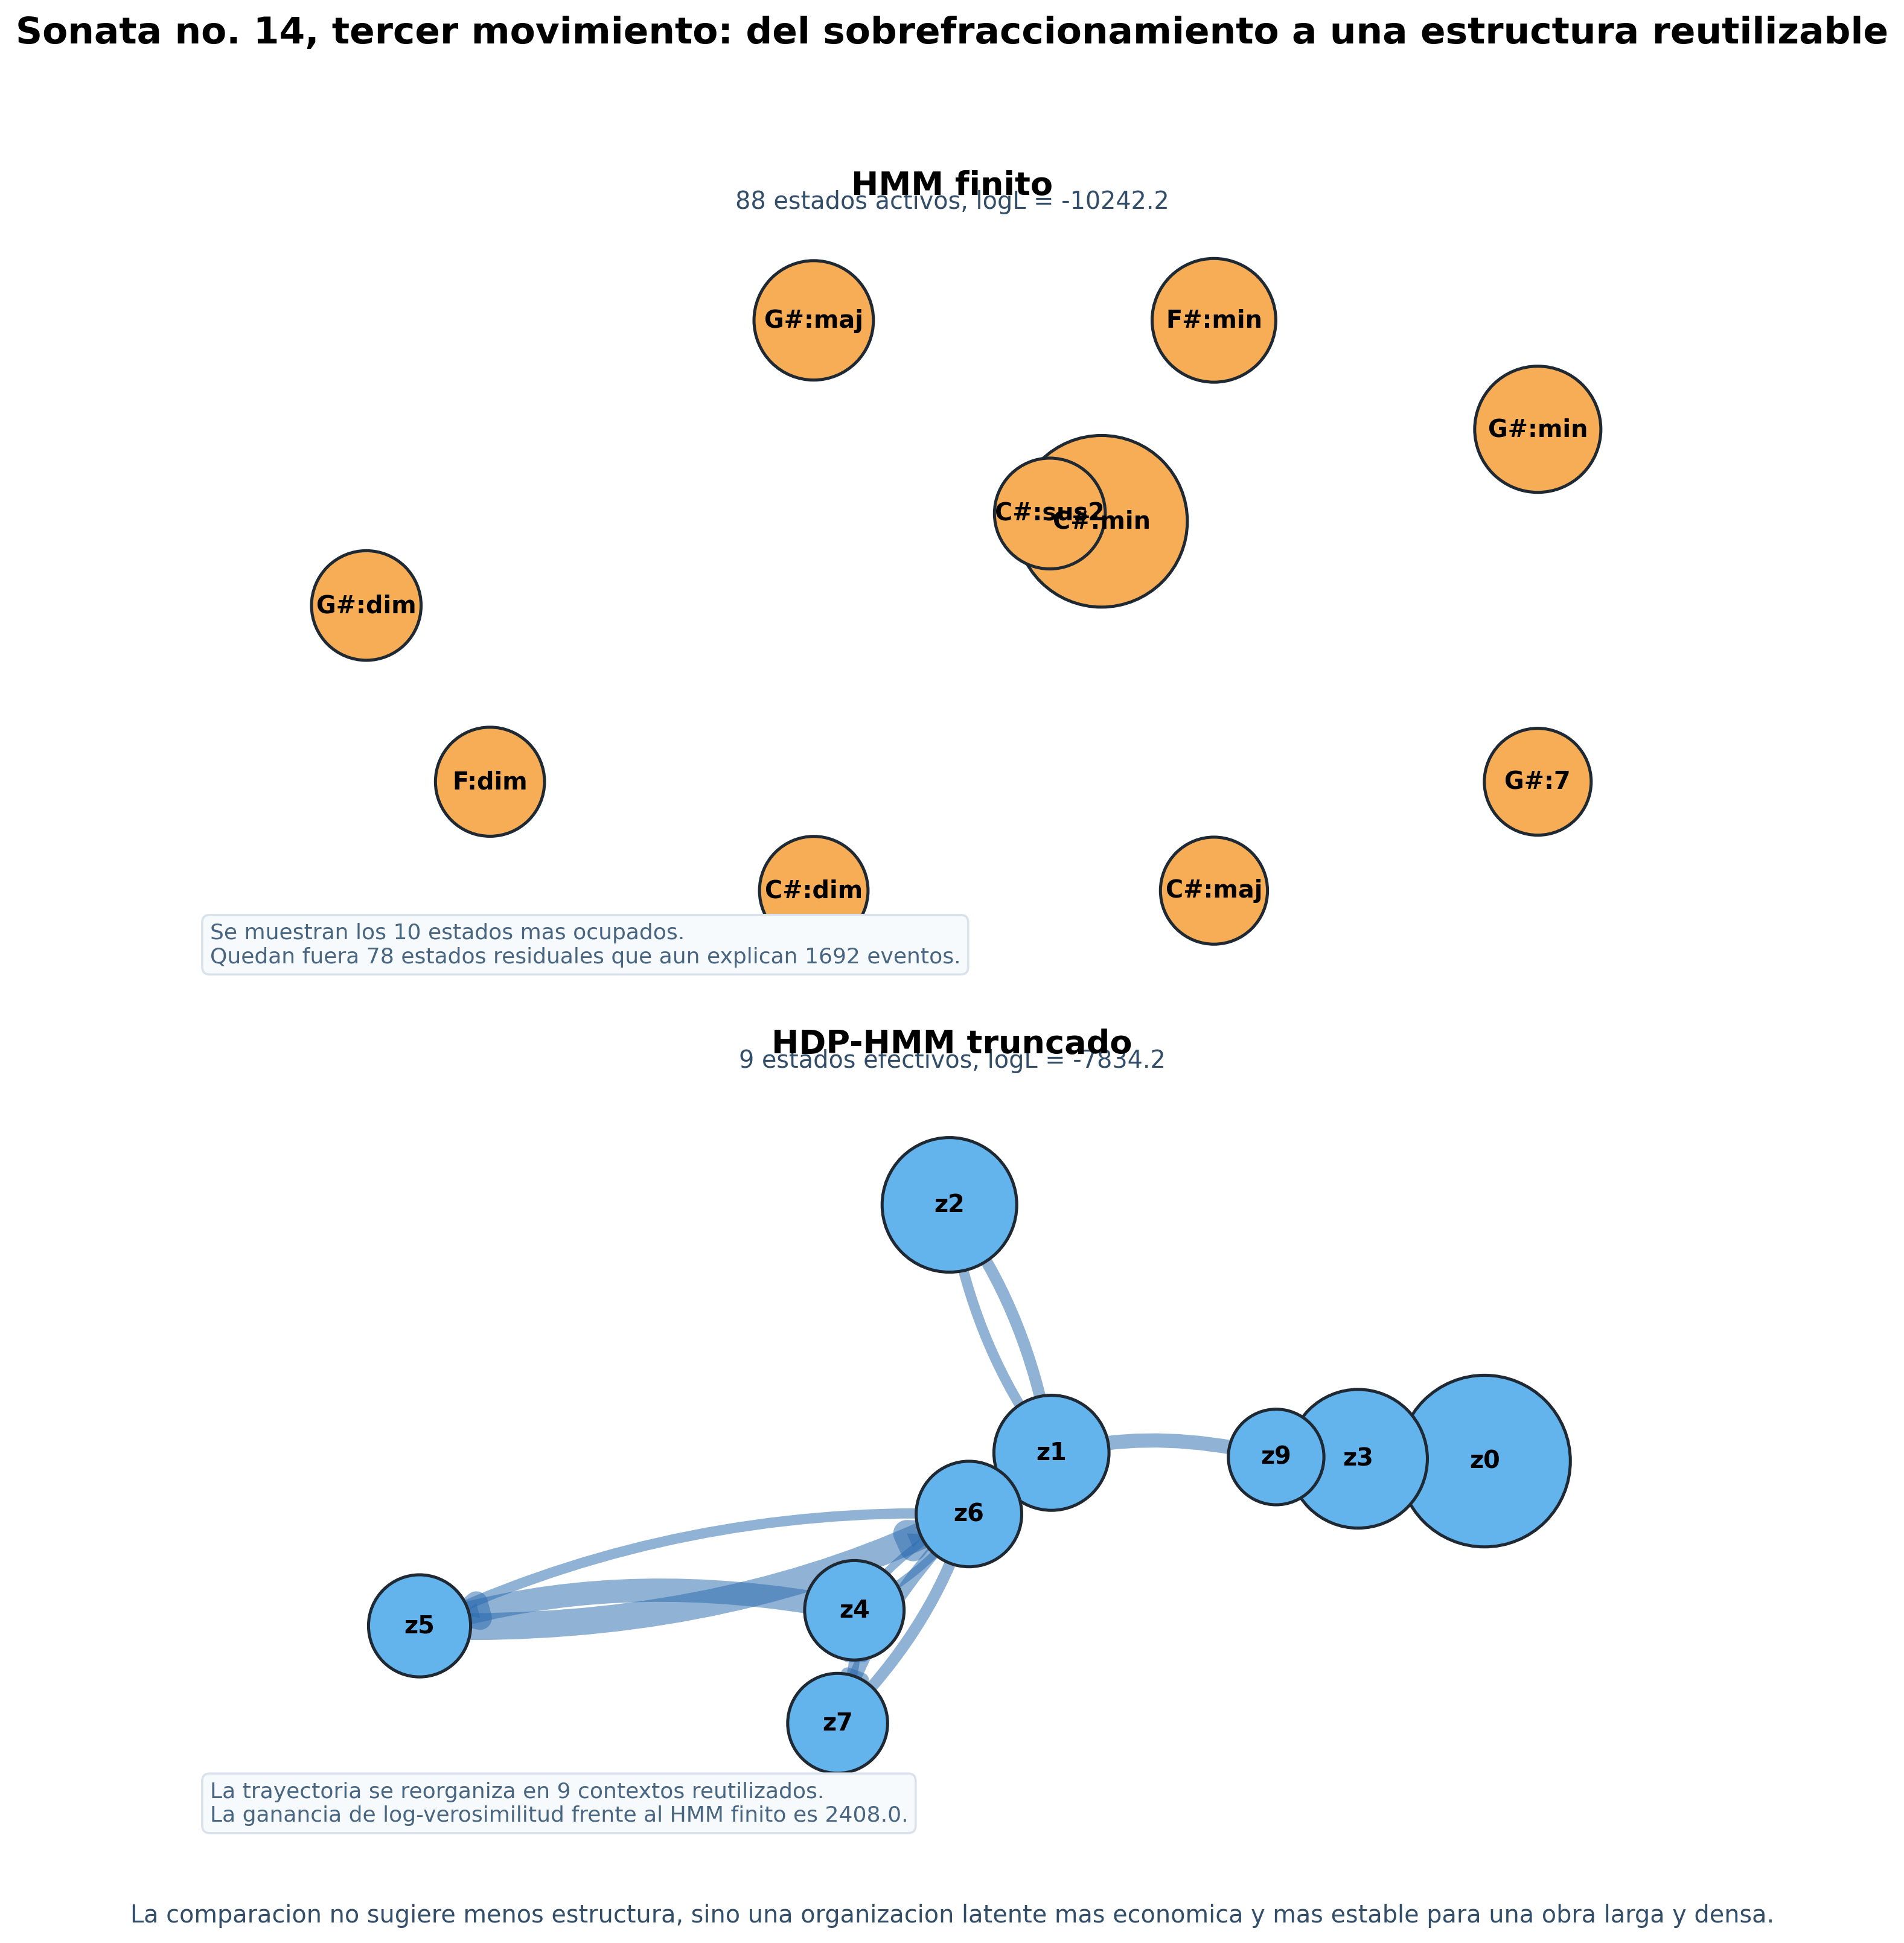
\includegraphics[width=\textwidth]{figures/chapter3/single_anchor_transition_comparison.png}
\caption{Obra ancla del capítulo. El HMM finito sobrefragmenta la trayectoria en una nube de estados activos, mientras que el HDP-HMM truncado reorganiza la misma secuencia en un conjunto mucho más compacto de contextos reutilizados.}
\label{fig:single-anchor-graph}
\end{figure}

Introducido el caso singular, el argumento necesita un control intermedio antes de generalizar al multicorpus. Por ello se conserva el caso base del capítulo como una escala reproducible de comparación: primero una obra difícil, después un subconjunto clásico pequeño y, sólo al final, el corpus heterogéneo de mayor tamaño.

\subsection{Resultados sobre un subconjunto clásico}

La evaluación comparativa se realizó sobre un subconjunto clásico limitado para mantener control experimental. La observación utilizada fue la clase de altura y el modelo truncado se ajustó con $K=12$, $\alpha=8$, $\alpha_0=4$, $\gamma=2$, $\eta=1$, $\kappa=0$, veinte iteraciones totales, diez de \emph{burn-in} y semilla igual a $7$. La Tabla~\ref{tab:corpus-clasico-limitado} resume las seis piezas breves utilizadas como base reproducible de comparación.

\begin{table}[H]
\centering
\footnotesize
\setlength{\tabcolsep}{4pt}
\begin{tabular}{@{}p{5.5cm}p{2.8cm}rr@{}}
\hline
Obra & Compositor & Notas & Compases \\
\hline
Cumpleanos feliz (Do mayor) & Tradicional & 37 & 8 \\
Oda a la alegria (variacion facil) & Desconocido & 87 & 17 \\
Para Elisa (version facil) & Beethoven & 103 & 22 \\
Cumpleanos feliz (arreglo) & Manjuprasad & 106 & 19 \\
Para Elisa (piano para principiantes) & Beethoven & 149 & 23 \\
Greensleeves & Desconocido & 166 & 33 \\
\hline
\end{tabular}

\caption{Subconjunto clásico limitado utilizado para la comparación reproducible entre el HMM finito y el HDP-HMM truncado.}
\label{tab:corpus-clasico-limitado}
\end{table}

La Tabla~\ref{tab:resumen-resultados-clasicos} condensa el resultado central: en las seis obras, el modelo truncado obtiene una log-verosimilitud superior a la del HMM finito. La ganancia media es de $92.970$ unidades, la mediana de $98.739$ y el número medio de estados efectivos del HDP-HMM truncado es menor que el número medio de estados activos del baseline finito.

\begin{table}[H]
\centering
\small
\begin{tabular}{lr}
\hline
Metrica & Valor \\
\hline
Obras comparables & 6 \\
Casos en que el HDP-HMM truncado mejora & 6 \\
Casos en que el HDP-HMM truncado empeora & 0 \\
Empates & 0 \\
Ganancia media de log-verosimilitud & 92.970 \\
Ganancia mediana de log-verosimilitud & 98.739 \\
Media de log-verosimilitud del HMM finito & -267.685 \\
Media de log-verosimilitud del HDP-HMM truncado & -174.715 \\
Estados activos medios del HMM finito & 10.833 \\
Estados efectivos medios del HDP-HMM truncado & 6.667 \\
\hline
\end{tabular}

\caption{Resumen agregado de la comparación entre el HMM finito y el HDP-HMM truncado sobre el subconjunto clásico limitado.}
\label{tab:resumen-resultados-clasicos}
\end{table}

La evidencia por obra aparece en la Tabla~\ref{tab:resultados-por-obra}. Dado que este experimento intermedio fue diseñado como control reproducible y no como corpus amplio, la tabla contiene sólo seis piezas. La magnitud de la mejora varía, pero el patrón es uniforme: ninguna favorece al modelo finito. Incluso en este repertorio sencillo, permitir que el número efectivo de estados se ajuste a la obra produce una ventaja estadística tangible.

\begin{table}[H]
\centering
\footnotesize
\setlength{\tabcolsep}{4pt}
\begin{tabular}{@{}p{4.2cm}p{2.1cm}rrrr@{}}
\hline
Obra & Compositor & Notas & $\log L_{fin}$ & $\log L_{hdp}$ & $\Delta \log L$ \\
\hline
Cumpleaños feliz (Do mayor) & Tradicional & 37 & -91.575 & -63.314 & 28.261 \\
Oda a la alegría (variación fácil) & Desconocido & 87 & -215.515 & -121.835 & 93.680 \\
Para Elisa (versión fácil) & Beethoven & 103 & -255.714 & -158.149 & 97.565 \\
Cumpleaños feliz (arreglo) & Manjuprasad & 106 & -262.027 & -162.114 & 99.914 \\
Greensleeves & Desconocido & 166 & -411.682 & -308.600 & 103.083 \\
Para Elisa (piano para principiantes) & Beethoven & 149 & -369.596 & -234.276 & 135.321 \\
\hline
\end{tabular}

\caption{Comparación por obra en las seis piezas del subconjunto clásico. La ganancia se calcula como la diferencia \mbox{HDP-HMM truncado $-$ HMM finito}.}
\label{tab:resultados-por-obra}
\end{table}

La Figura~\ref{fig:logverosimilitud-clasica} confirma visualmente el mismo patrón: todas las obras quedan del lado favorable al HDP-HMM truncado y la distribución agregada de log-verosimilitud también se desplaza en su favor.

\begin{figure}[H]
\centering
\begin{subfigure}[t]{0.88\textwidth}
\centering
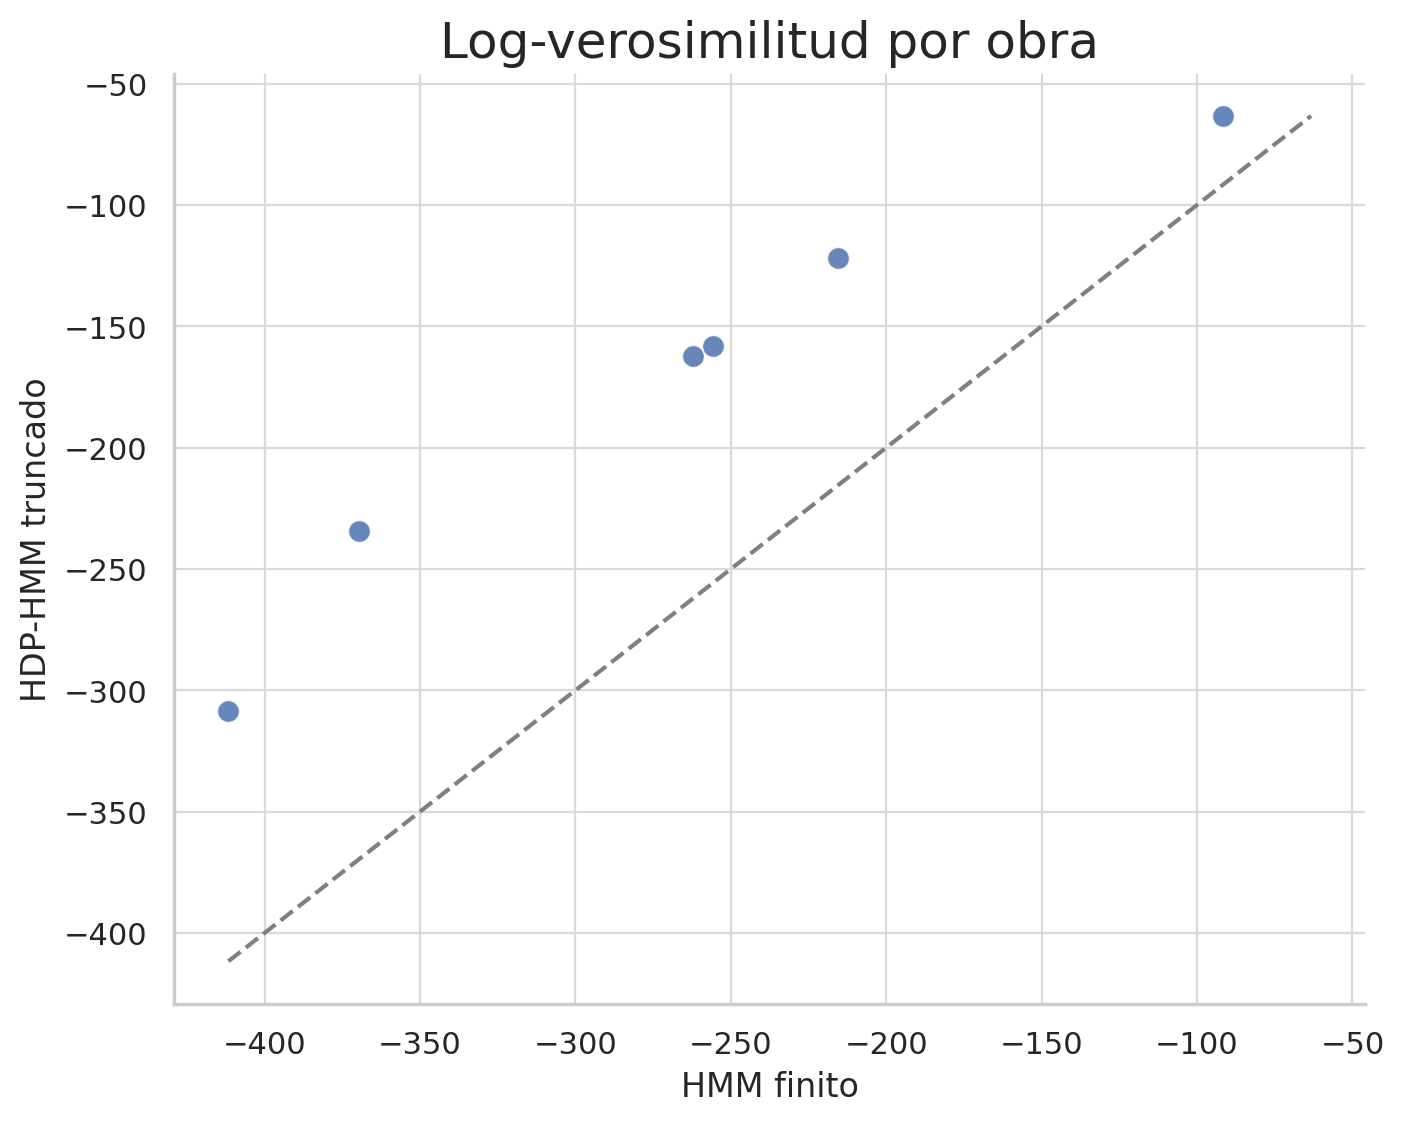
\includegraphics[width=\linewidth]{figures/chapter3/classic_log_likelihood_scatter.png}
\caption{Comparación de log-verosimilitud por obra.}
\end{subfigure}

\medskip
\begin{subfigure}[t]{0.88\textwidth}
\centering
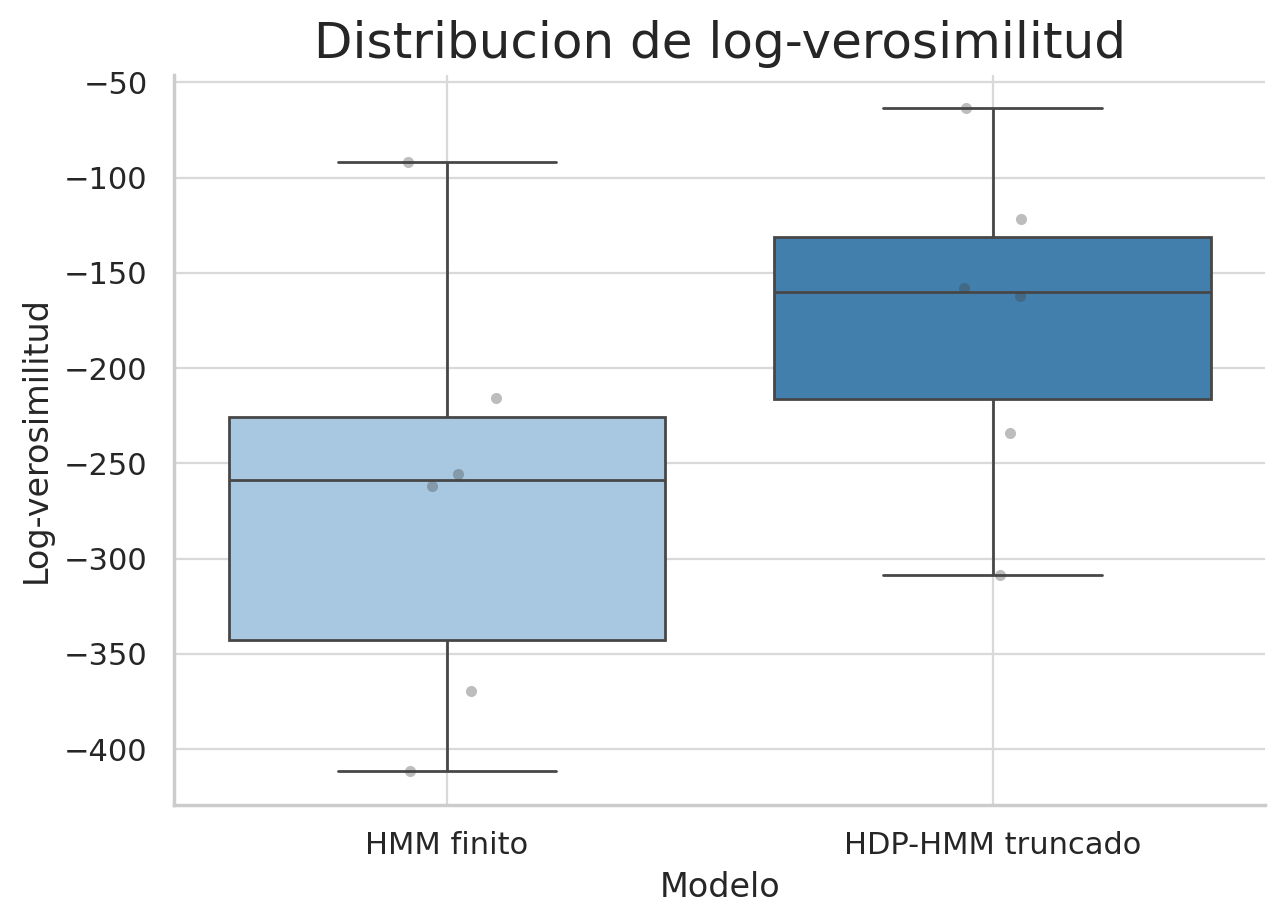
\includegraphics[width=\linewidth]{figures/chapter3/classic_log_likelihood_boxplot.png}
\caption{Distribución agregada de log-verosimilitud por modelo.}
\end{subfigure}
\caption{Lectura visual del ajuste probabilístico en el subconjunto clásico limitado. En ambos paneles, el desplazamiento favorece al HDP-HMM truncado.}
\label{fig:logverosimilitud-clasica}
\end{figure}

La Figura~\ref{fig:ganancia-y-complejidad-clasica} añade el segundo punto importante: la mejora no proviene de inflar indiscriminadamente la complejidad. El HDP-HMM truncado obtiene mejor ajuste y, al mismo tiempo, usa menos estados efectivos que el HMM finito.

\begin{figure}[H]
\centering
\begin{subfigure}[t]{0.88\textwidth}
\centering
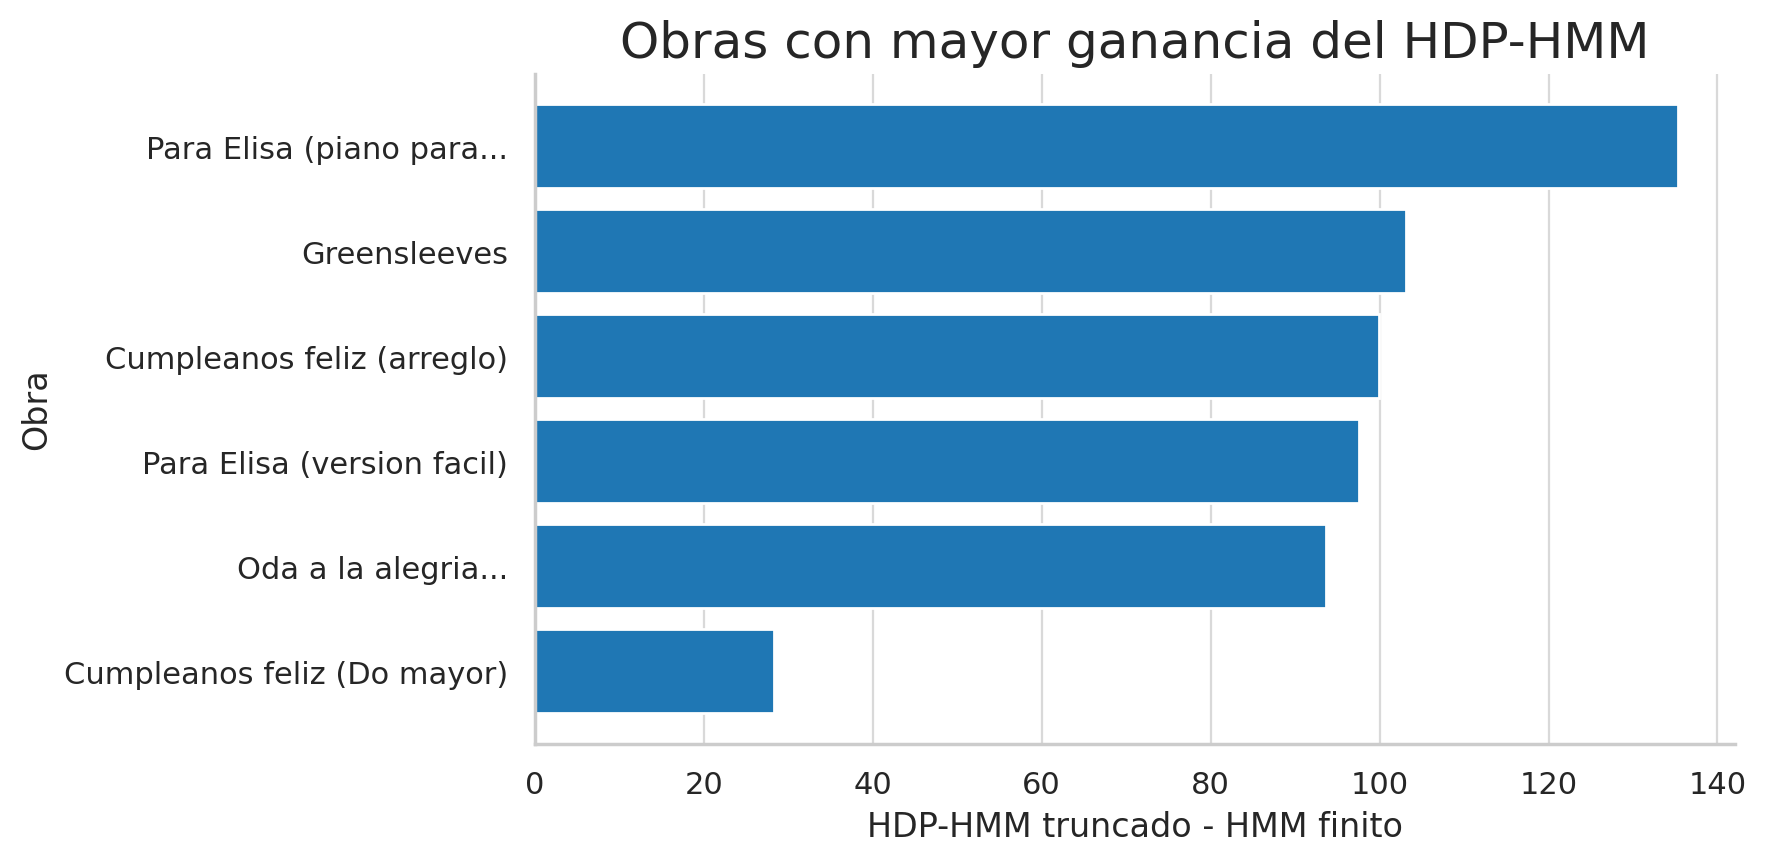
\includegraphics[width=\linewidth]{figures/chapter3/classic_log_likelihood_gain_by_piece.png}
\caption{Ganancia de log-verosimilitud por obra.}
\end{subfigure}

\medskip
\begin{subfigure}[t]{0.88\textwidth}
\centering
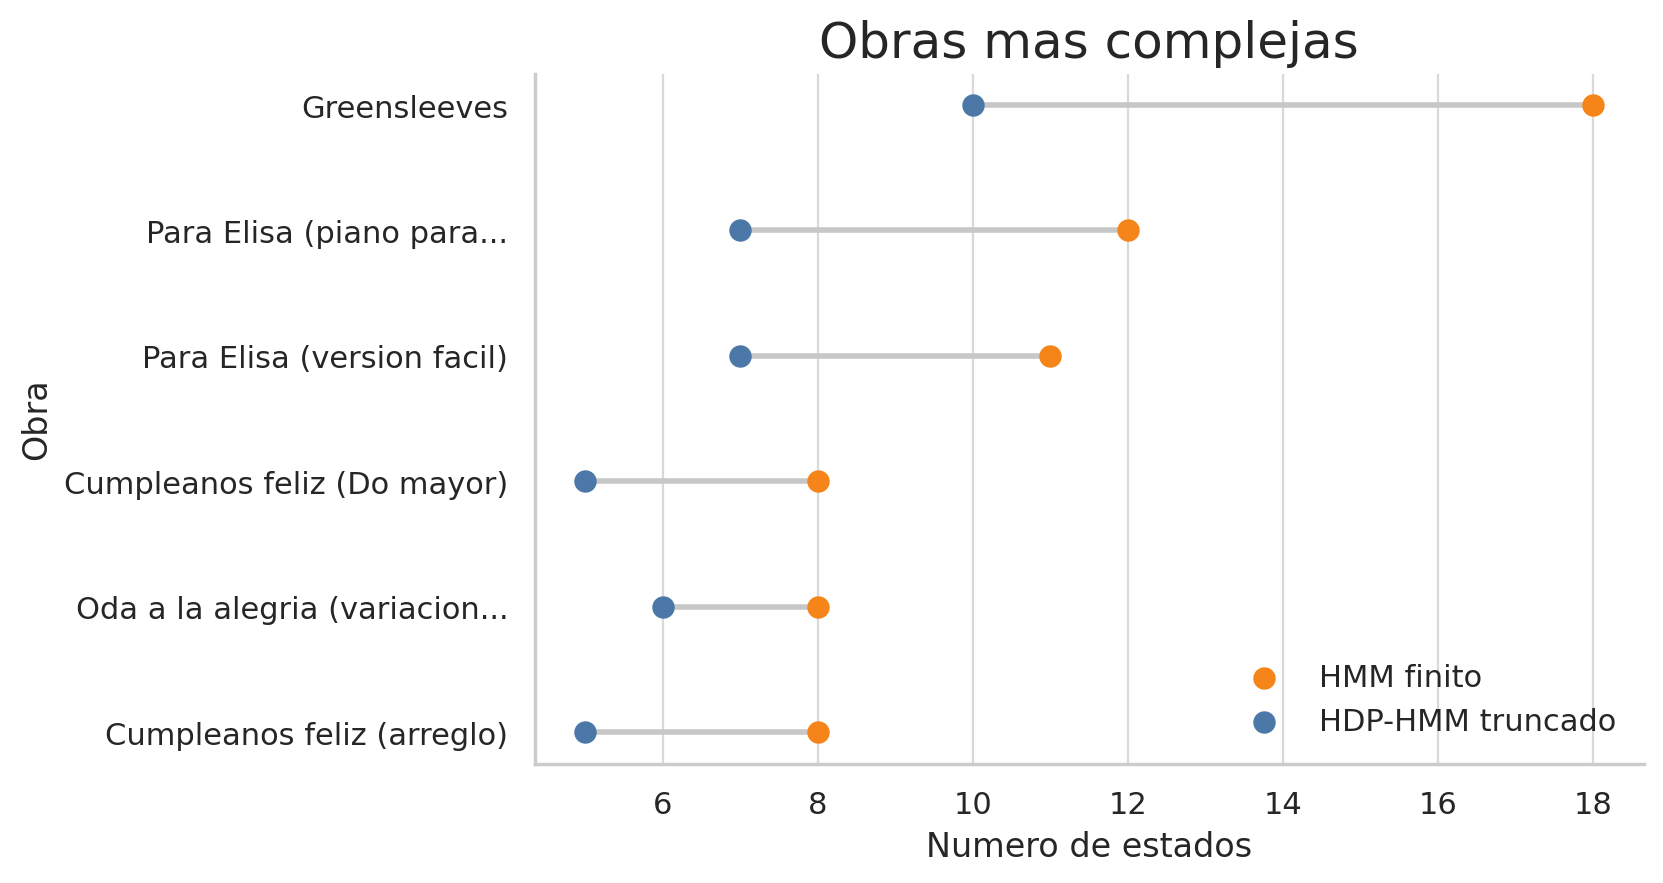
\includegraphics[width=\linewidth]{figures/chapter3/classic_state_counts_by_piece.png}
\caption{Comparación del número de estados por obra.}
\end{subfigure}
\caption{Descomposición visual de la ventaja del HDP-HMM truncado. El panel izquierdo mide la ganancia en ajuste y el derecho compara la complejidad latente efectiva de ambos modelos.}
\label{fig:ganancia-y-complejidad-clasica}
\end{figure}

Estos resultados deben leerse con cautela: el subconjunto es pequeño y la log-verosimilitud no agota la calidad musicológica de una segmentación latente. Su función dentro del capítulo es más específica: servir de puente entre la obra ancla y el multicorpus. Aun así, la evidencia basta para sostener la conclusión metodológica de esta sección: cuando no se fija \emph{ex ante} el número efectivo de estados, la aproximación truncada al iHMM mejora el ajuste y mantiene una complejidad posterior contenida.

\subsection{Resultados sobre el corpus extendido}

Una vez establecida la ventaja del modelo truncado en una obra exigente y en un subconjunto clásico controlado, conviene preguntar si esa ventaja se mantiene al ampliar el repertorio. Para ello se construyó un corpus extendido con dos fuentes: repertorio occidental etiquetado como \texttt{MuseTrainer} y material de tradición makam procedente de \texttt{SymbTr}. La Tabla~\ref{tab:corpus-extendido} resume su composición. El interés de esta ampliación no es homogeneizar ambos repertorios, sino probar la estabilidad del modelo cuando cambia de manera significativa el entorno estilístico.

\begin{table}[H]
\centering
\footnotesize
\setlength{\tabcolsep}{4pt}
\begin{tabular}{@{}p{2.2cm}p{8.2cm}r@{}}
\hline
Fuente & Perfil del material incorporado & Obras \\
\hline
MuseTrainer & Repertorio tonal occidental de orientacion pedagogica y clasica, con piezas breves y medianas en formato MusicXML. & 69 \\
SymbTr & Repertorio de musica artistica turca; el adaptador conserva metadatos de \emph{makam}, \emph{usul} y forma para preservar la procedencia modal. & 100 \\
\hline
Total & Corpus extendido usado para evaluar la estabilidad del modelo bajo mayor heterogeneidad estilistica. & 169 \\
\hline
\end{tabular}

\caption{Composición del corpus extendido utilizado en la comparación multicorpus.}
\label{tab:corpus-extendido}
\end{table}

De las $169$ obras catalogadas, $168$ pudieron correrse en la evaluación multicorpus y $167$ quedaron comparables entre ambos modelos; en la corrida base una obra de Mozart no entró al lote final y una pieza de Brahms arrojó un error de ejecución. Aun con esa salvedad, la evidencia es nítida. La Tabla~\ref{tab:resultados-multicorpus} muestra que el HDP-HMM truncado mejora la log-verosimilitud en las $167$ obras comparables. La ganancia media global asciende a $452.751$ unidades y la mediana a $377.039$, mientras que el número medio de estados efectivos del HDP-HMM truncado se mantiene cerca de $8$ frente a más de $32$ estados activos del HMM finito.

\begin{table}[H]
\centering
\footnotesize
\setlength{\tabcolsep}{4pt}
\begin{tabular}{lrrrrrrr}
\hline
Fuente & Obras & $\overline{\Delta \log L}$ & $\widetilde{\Delta \log L}$ & $\overline{\log L}_{fin}$ & $\overline{\log L}_{hdp}$ & $\overline{K}_{fin}$ & $\overline{K}_{hdp}$ \\
\hline
Global & 167 & 452.751 & 377.039 & -1598.180 & -1145.429 & 32.162 & 8.222 \\
MuseTrainer & 67 & 585.443 & 467.011 & -2667.850 & -2082.406 & 46.418 & 8.731 \\
SymbTr & 100 & 363.848 & 336.438 & -881.502 & -517.654 & 22.610 & 7.880 \\
\hline
\end{tabular}

\caption{Resumen agregado de la comparación entre el HMM finito y el HDP-HMM truncado sobre el corpus extendido. La mejora se calcula como \mbox{HDP-HMM truncado $-$ HMM finito}.}
\label{tab:resultados-multicorpus}
\end{table}

Como el multicorpus reúne $167$ comparaciones válidas, una tabla exhaustiva por obra rompería el flujo del capítulo. Por ello, la Tabla~\ref{tab:resultados-multicorpus-muestra} presenta una muestra representativa balanceada entre ambas fuentes y distribuida a lo largo de distintos tamaños de pieza. Aun en esa lectura parcial, la ventaja del HDP-HMM truncado se mantiene.

\begin{table}[H]
\centering
\footnotesize
\setlength{\tabcolsep}{4pt}
\begin{tabular}{@{}p{1.7cm}p{4.6cm}rrrr@{}}
\hline
Fuente & Obra & Notas & $\log L_{fin}$ & $\log L_{hdp}$ & $\Delta \log L$ \\
\hline
MuseTrainer & Cumpleanos feliz (Do mayor) & 37 & -91.575 & -62.059 & 29.516 \\
MuseTrainer & Danse Villageoise & 519 & -1286.408 & -887.259 & 399.149 \\
MuseTrainer & Clair de Lune & 1220 & -3020.550 & -2421.226 & 599.324 \\
MuseTrainer & Sonata no. 14, tercer movimiento & 4133 & -10242.186 & -7549.906 & 2692.280 \\
SymbTr & Acemkürdî Aranağme (Düyek) & 58 & -144.102 & -66.151 & 77.951 \\
SymbTr & Aldanma Dünya Varına & 266 & -660.614 & -349.715 & 310.898 \\
SymbTr & Yıllar Sonra Rastladım... & 417 & -1035.314 & -546.391 & 488.922 \\
SymbTr & Âşık-I Ger & 1135 & -2815.965 & -1841.559 & 974.407 \\
\hline
\end{tabular}

\caption{Muestra representativa de resultados por obra en el corpus extendido. Se incluyen ejemplos de \texttt{MuseTrainer} y \texttt{SymbTr} para mostrar la estabilidad del patrón fuera del subconjunto clásico.}
\label{tab:resultados-multicorpus-muestra}
\end{table}

La Figura~\ref{fig:logverosimilitud-multicorpus} muestra visualmente la estabilidad de este resultado: las obras quedan del lado favorable al HDP-HMM truncado y la distribución agregada de log-verosimilitud también se desplaza de forma consistente.

\begin{figure}[H]
\centering
\begin{subfigure}[t]{0.88\textwidth}
\centering
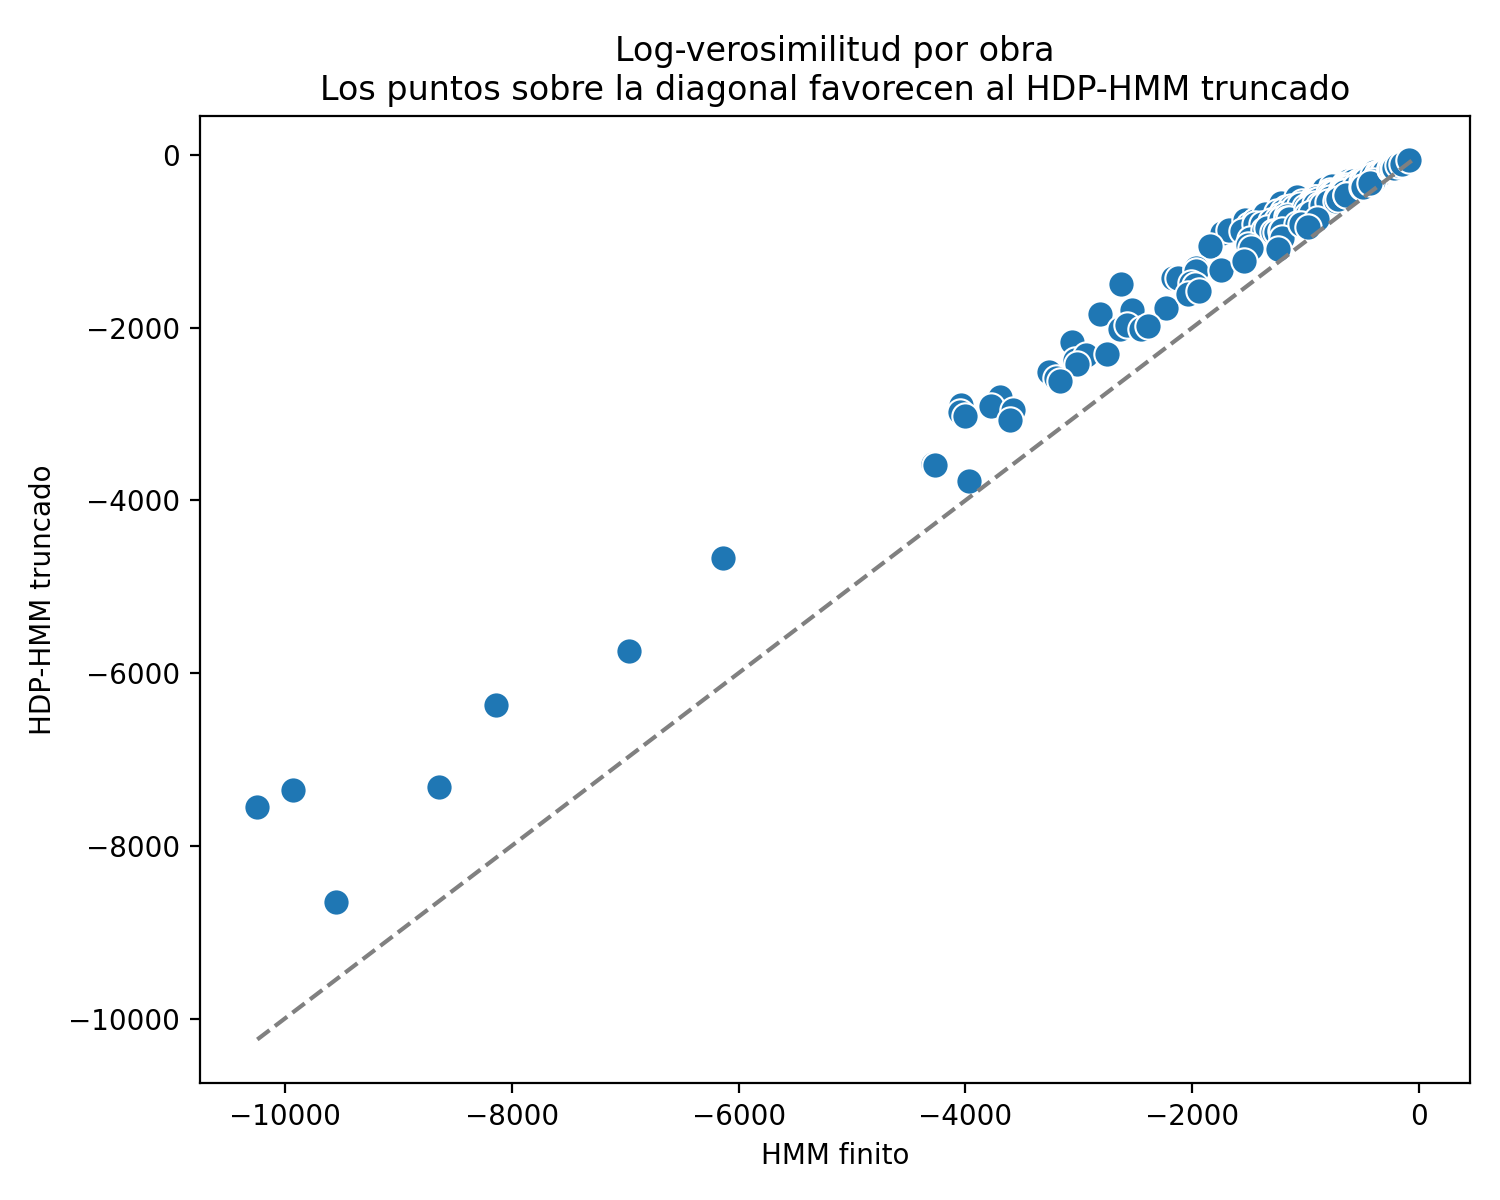
\includegraphics[width=\linewidth]{figures/chapter3/multicorpus_log_likelihood_scatter.png}
\caption{Comparación de log-verosimilitud por obra en el corpus extendido.}
\end{subfigure}

\medskip
\begin{subfigure}[t]{0.88\textwidth}
\centering
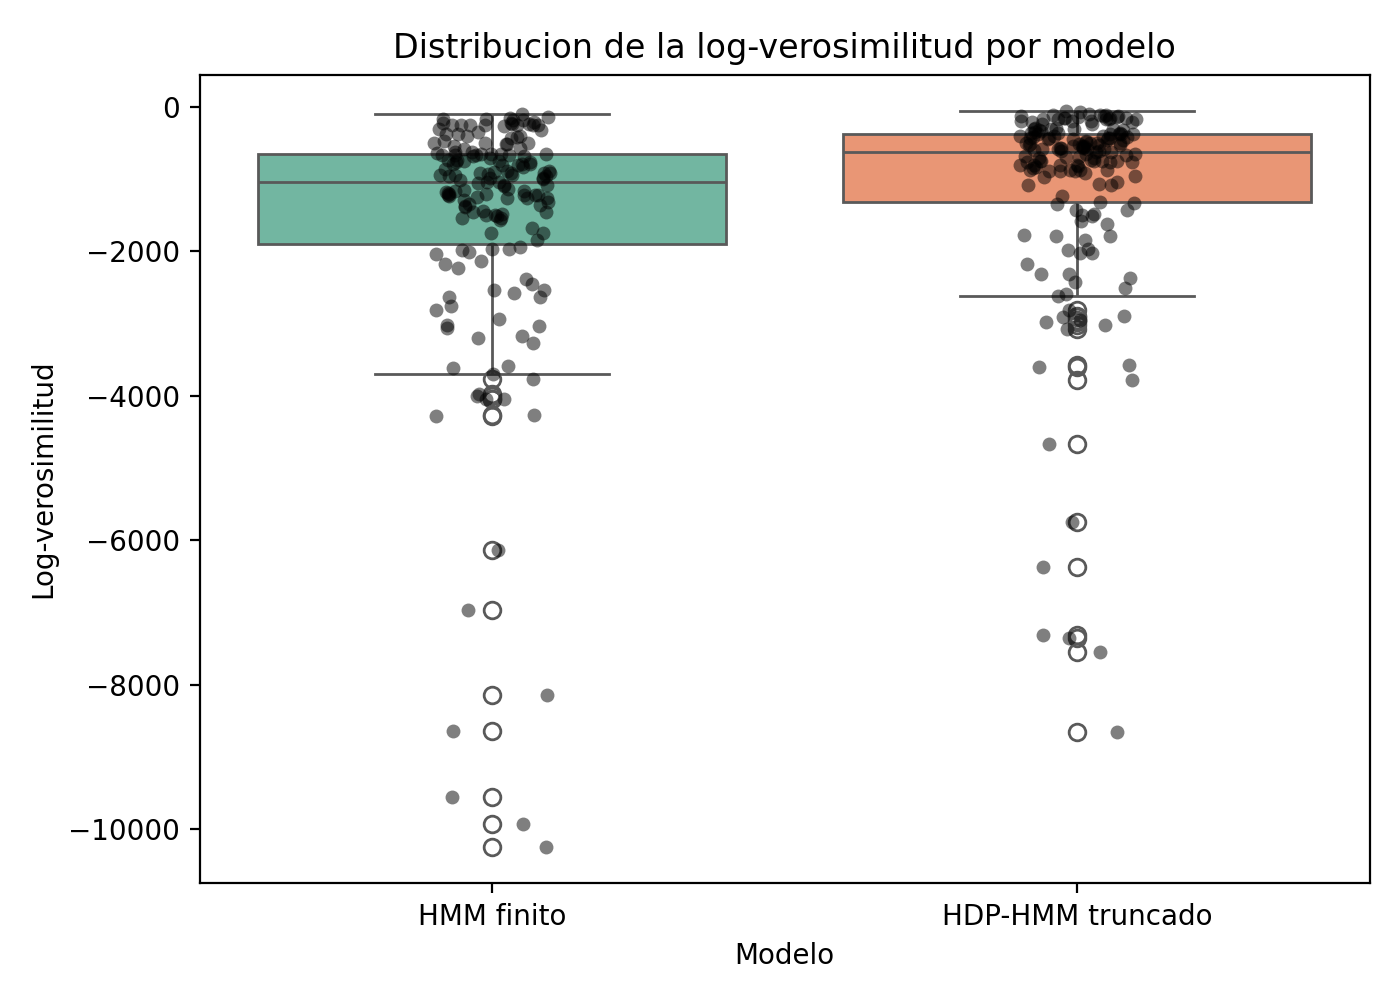
\includegraphics[width=\linewidth]{figures/chapter3/multicorpus_log_likelihood_boxplot.png}
\caption{Distribución agregada de log-verosimilitud por modelo.}
\end{subfigure}
\caption{Lectura visual del ajuste probabilístico sobre el corpus extendido. En ambos paneles, el desplazamiento favorece al HDP-HMM truncado.}
\label{fig:logverosimilitud-multicorpus}
\end{figure}

La Figura~\ref{fig:ganancia-y-complejidad-multicorpus} refuerza la misma lectura: la ganancia de log-verosimilitud es uniformemente positiva y el modelo truncado mantiene una ocupación efectiva de estados mucho más contenida que la del HMM finito.

\begin{figure}[H]
\centering
\begin{subfigure}[t]{0.88\textwidth}
\centering
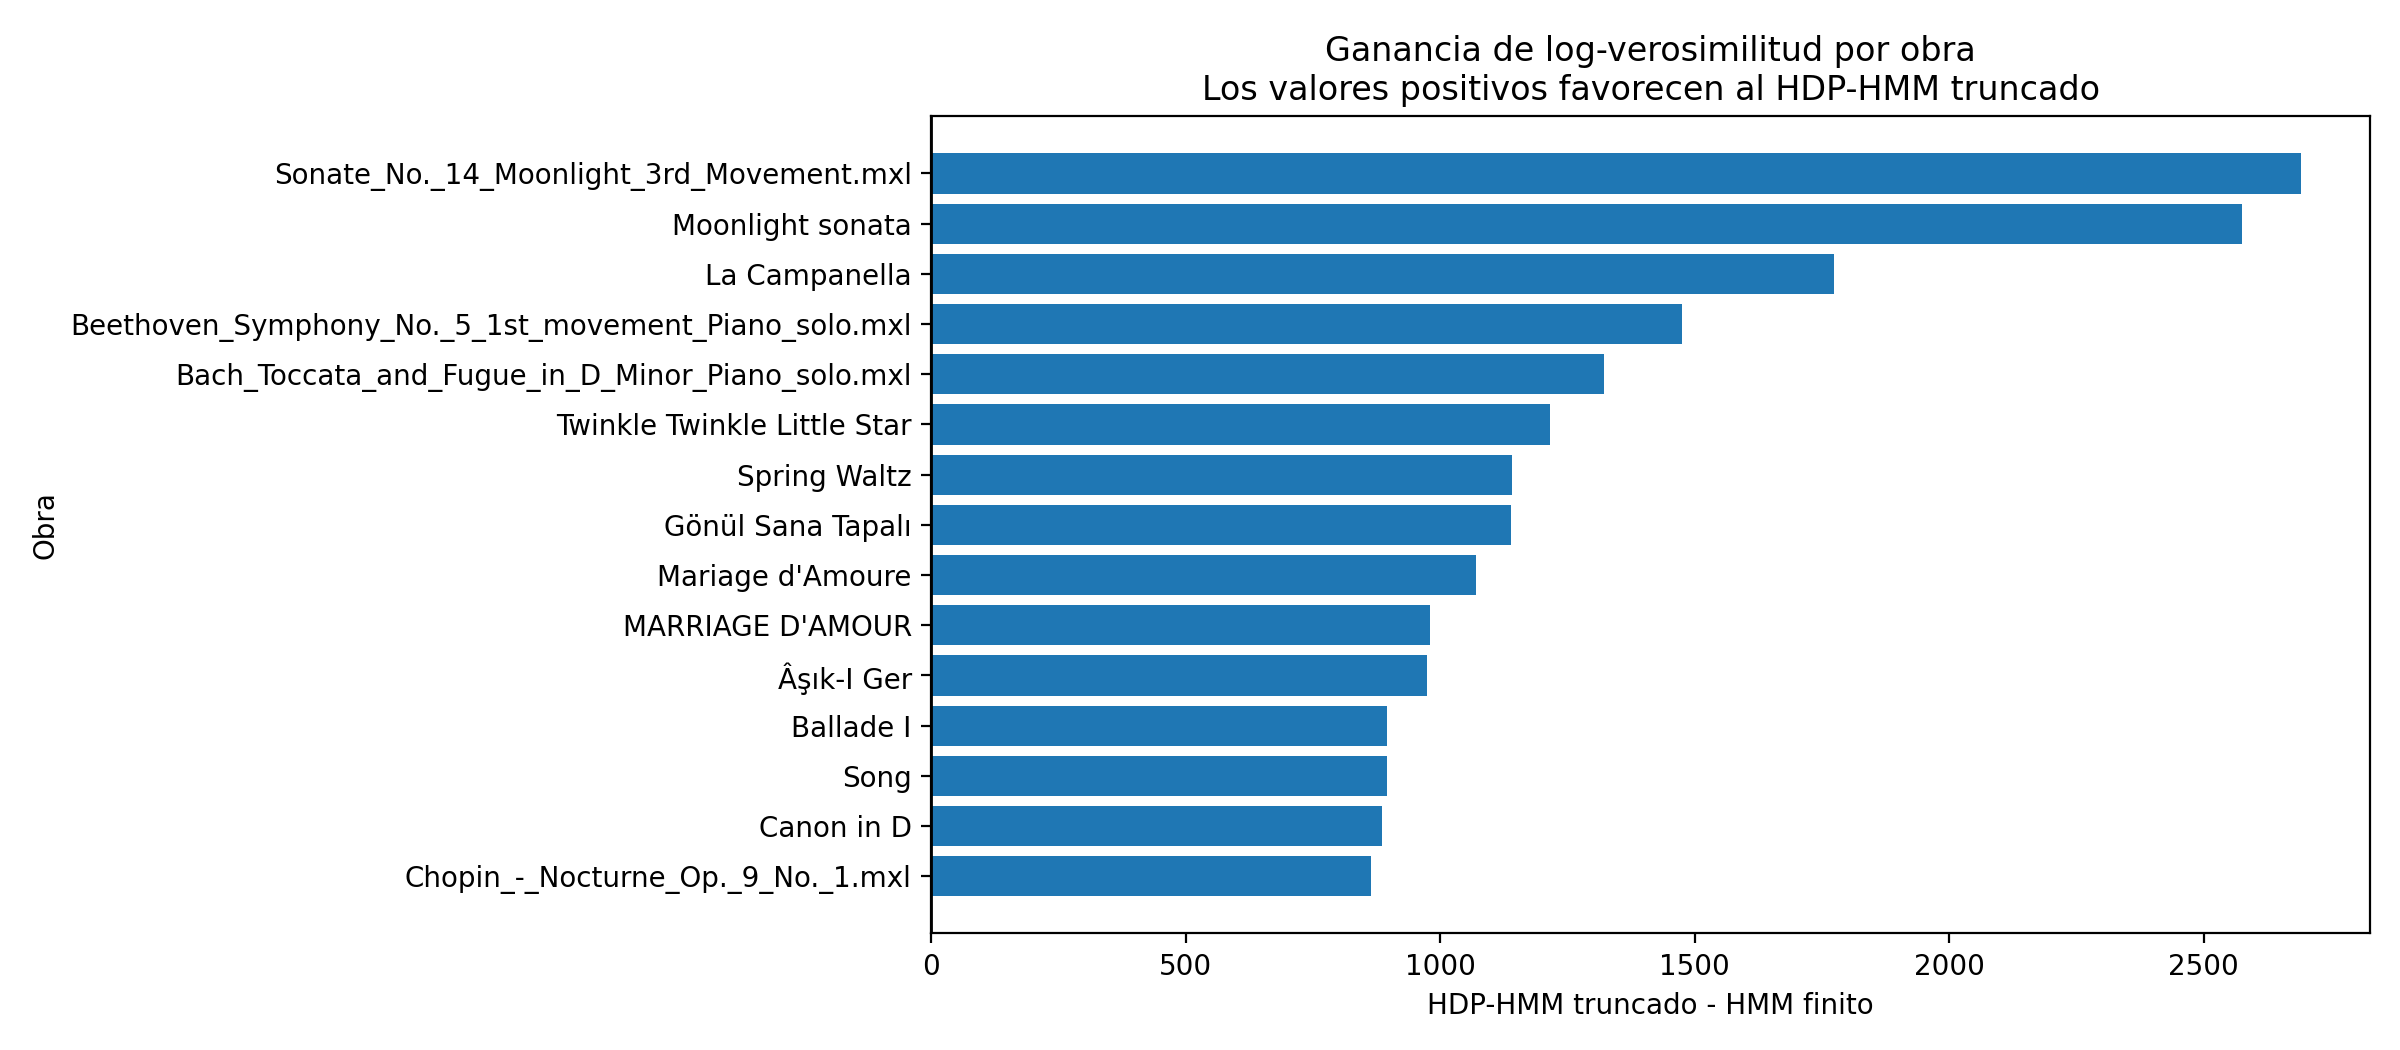
\includegraphics[width=\linewidth]{figures/chapter3/multicorpus_log_likelihood_gain_by_piece.png}
\caption{Ganancia de log-verosimilitud por obra.}
\end{subfigure}

\medskip
\begin{subfigure}[t]{0.88\textwidth}
\centering
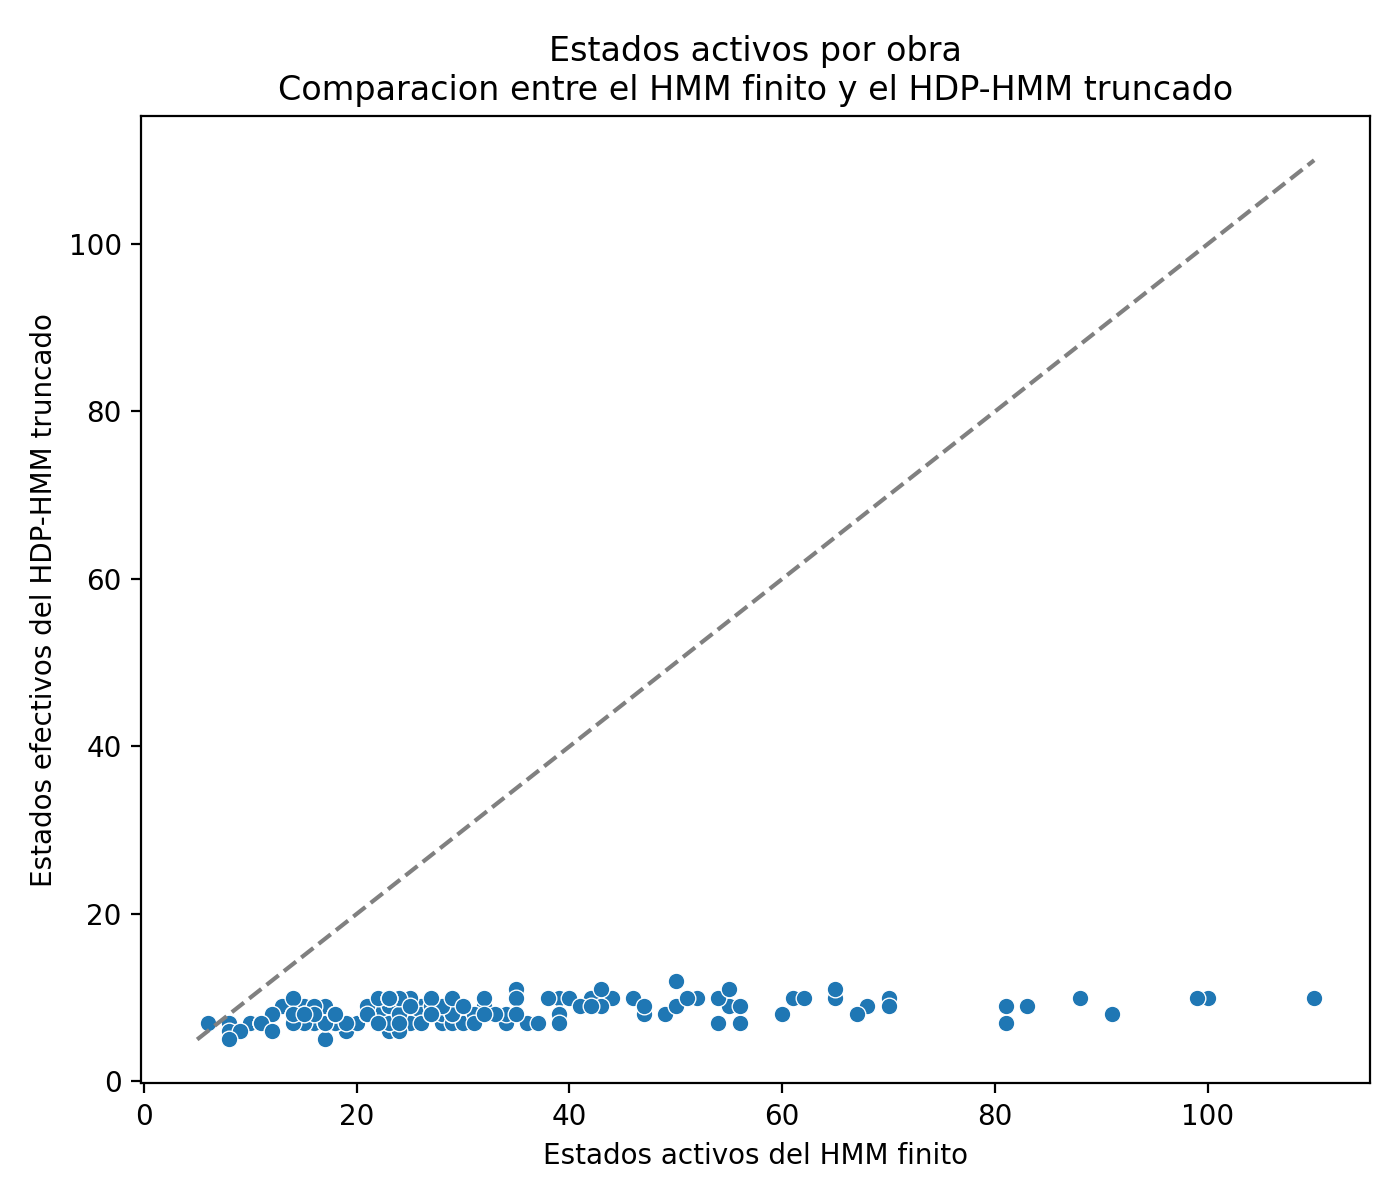
\includegraphics[width=\linewidth]{figures/chapter3/multicorpus_state_counts_scatter.png}
\caption{Comparación del número de estados utilizados por ambos modelos.}
\end{subfigure}
\caption{Ganancia y complejidad latente en el corpus extendido. El HDP-HMM truncado mejora el ajuste y, al mismo tiempo, mantiene una ocupación efectiva de estados mucho más contenida.}
\label{fig:ganancia-y-complejidad-multicorpus}
\end{figure}

La lectura crítica de esta evidencia exige distinguir entre mejora estadística y superioridad musicológica en sentido fuerte. En \texttt{SymbTr}, por ejemplo, la mejora no prueba que el vocabulario finito de referencia capture adecuadamente la teoría musical nativa del corpus; sí muestra, en cambio, que la aproximación truncada al modelo infinito es más robusta cuando el repertorio se vuelve heterogéneo. En conjunto, el corpus extendido fortalece la conclusión central del capítulo: truncar el iHMM no sólo vuelve viable la inferencia, sino que ofrece una realización empíricamente estable del principio no paramétrico, con mejor ajuste y complejidad efectiva menor.

    \chapter{Comparación final entre HMM, HDP-HMM y Transformer}
\label{chap:comparacion-final}

Los capítulos anteriores desarrollaron dos familias de modelos probabilísticos para análisis musical simbólico. Por una parte, el HMM finito proporcionó un marco interpretable para describir la relación entre estados latentes y secuencias observables. Por otra, el HDP-HMM permitió relajar la fijación \emph{a priori} del número de estados y ofreció una alternativa no paramétrica para capturar una estructura latente más flexible. El paso natural que sigue consiste en contrastar estos enfoques con una familia distinta de modelos secuenciales: los transformadores causales aplicados a predicción del siguiente evento musical.

La motivación de este capítulo no es asumir desde el inicio que el transformador deba reemplazar a los modelos markovianos. El problema relevante es más preciso. Si los transformadores exigen una infraestructura experimental más amplia, mayor costo de cómputo, decisiones de representación más delicadas y una validación más extensa, entonces la comparación adecuada no debe limitarse a una sola métrica predictiva. La pregunta central es si ese incremento de complejidad produce una mejora sustancial, consistente y metodológicamente defendible para el análisis musical considerado en esta tesis.

Este capítulo se concibe como un capítulo de cierre comparativo. Su función es integrar, en un mismo marco, cuatro dimensiones que suelen evaluarse por separado: capacidad predictiva, costo computacional, costo de desarrollo e interpretabilidad analítica. En lugar de tratar la comparación como una oposición simplista entre ``modelo clásico'' y ``modelo moderno'', se propone una evaluación balanceada de compromisos. El HMM y el HDP-HMM parten de una estructura latente explícita y musicalmente interpretable; el transformador, en cambio, desplaza parte de la carga modelística hacia la representación de entrada, la escala de entrenamiento y la capacidad del modelo para explotar dependencias de contexto más largas.

La utilidad de una comparación de este tipo es doble. Desde el punto de vista metodológico, permite decidir si la ampliación de infraestructura justifica su incorporación al programa de investigación. Desde el punto de vista sustantivo, permite determinar si la mejora cuantitativa del transformador, en caso de aparecer, va acompañada de una ganancia real para la comprensión del fenómeno musical y no sólo de un aumento de capacidad estadística difícil de interpretar.

\section{Pregunta de comparación y criterio de decisión}

La pregunta guía de este capítulo puede formularse así:
\begin{quote}
\emph{¿La complejidad adicional requerida por un transformador causal para modelar secuencias musicales simbólicas produce una mejora suficiente frente al HMM finito y al HDP-HMM truncado como para justificar su adopción dentro de esta línea de trabajo?}
\end{quote}

Responder esta pregunta exige evitar dos reduccionismos. El primero consiste en juzgar los modelos únicamente por su costo computacional, lo cual invisibiliza posibles mejoras reales en calidad predictiva o cobertura estructural. El segundo consiste en juzgarlos únicamente por la métrica final, como si una mejora marginal de \emph{perplexity} bastara para justificar un ecosistema experimental mucho más costoso y opaco. En esta tesis se adopta una posición intermedia: la comparación debe ser cuantitativa, pero también debe ser metodológicamente legible.

El criterio de decisión que guiará el análisis comparativo se articula en torno a cinco preguntas:
\begin{enumerate}
    \item ¿Qué modelo ofrece la mejor calidad predictiva global bajo condiciones de entrenamiento y evaluación comparables?
    \item ¿En qué subconjuntos del corpus se observan las mejoras y con qué estabilidad aparecen?
    \item ¿Qué costo computacional adicional exige cada mejora observada?
    \item ¿Qué costo de implementación, mantenimiento y experimentación requiere cada familia de modelos?
    \item ¿Qué tan interpretable sigue siendo el resultado desde el punto de vista musical?
\end{enumerate}

Estas preguntas delimitan una comparación costo-beneficio, no una competencia aislada de rendimiento.

\section{Dimensiones de costo relevantes}

Para comparar tecnologías de modelado secuencial en este contexto no basta medir tiempo total de entrenamiento. El costo aparece en varias capas, y cada una tiene consecuencias distintas para la práctica investigativa. En este capítulo se distinguen cinco dimensiones.

Primero, el \emph{costo de implementación} describe la cantidad de infraestructura adicional necesaria para poner en marcha una línea experimental. En los modelos HMM y HDP-HMM, buena parte del trabajo se concentra en fijar el espacio observable, la estructura latente y los procedimientos de inferencia. En el caso del transformador, el costo incluye además el diseño de representaciones simbólicas, perfiles de entrenamiento, trazabilidad de corridas, agregación de resultados, manejo de contextos y selección de hiperparámetros.

Segundo, el \emph{costo de experimentación} se refiere a la cantidad de corridas, ajustes y validaciones necesarias para llegar a un resultado confiable. Un HMM finito puede evaluarse con un número relativamente controlado de configuraciones. Un transformador, en cambio, suele requerir comparar representación, longitud de contexto, tamaño del modelo, regularización, estrategia de muestreo y criterios de selección de checkpoints.

Tercero, el \emph{costo computacional} incluye tiempo de ajuste, tiempo de evaluación, memoria, dependencia de hardware especializado y sensibilidad a la escala del corpus. Esta dimensión es importante porque una mejora cuantitativa modesta puede resultar poco defendible si sólo aparece a costa de un aumento pronunciado del presupuesto experimental.

Cuarto, el \emph{costo epistémico} alude a la pérdida potencial de interpretabilidad. Un HMM o un HDP-HMM permiten asociar estados latentes, transiciones y emisiones con hipótesis musicales identificables. Un transformador puede mejorar predicción sin ofrecer una estructura latente directamente comparable. La cuestión no es si esto lo invalida, sino cuánto encarece la tarea de justificar sus resultados en términos musicales.

Quinto, el \emph{costo de mantenimiento} describe la dificultad de sostener el pipeline a lo largo del tiempo. Un sistema experimental con muchos perfiles, scripts de agregación, artefactos de benchmarking y decisiones de infraestructura requiere más disciplina de documentación y más trabajo para conservar reproducibilidad.

En el estado actual del proyecto, este costo ya puede registrarse de manera concreta y no sólo con carácter hipotético. Para sostener la línea del transformador fue necesario separar explícitamente un \emph{baseline} conservador en CPU y un \emph{track} de investigación, introducir una representación simbólica más rica con silencios y posición métrica, incorporar sesgo posicional relativo, habilitar una ruta de atención acelerada con retorno seguro a la implementación conservadora y ampliar la batería de pruebas y de reportes reproducibles. Además, la comparación ya no se reduce a una corrida única: exige una suite canónica de corridas \emph{baseline} frente a \emph{research}, así como ablaciones de representación, posición y longitud de contexto. Nada de esto invalida al transformador, pero sí vuelve visible un hecho metodológico importante: aun antes de demostrar una mejora predictiva sustancial, la familia neuronal ya impone un costo de desarrollo y de mantenimiento claramente mayor que el requerido por los modelos probabilísticos.

\section{Diseño de comparación}

La comparación entre HMM, HDP-HMM y transformador se organizará sobre una batería canónica de corridas, construida para evitar evaluaciones anecdóticas. En el caso del transformador, esta batería debe distinguir explícitamente entre corridas de validación rápida y corridas destinadas a análisis formal. La batería actual ya puede describirse en dos capas:
\begin{enumerate}
    \item una capa histórica de referencia, formada por \texttt{cpu\_baseline\_smoke}, \texttt{cpu\_baseline\_full}, \texttt{research\_richer\_events\_smoke} y \texttt{research\_richer\_events\_full};
    \item una capa de ablaciones controladas, que separa representación, posición y contexto mediante familias específicas de corridas.
\end{enumerate}

En particular, la familia \texttt{research\_pitch\_duration} aísla el efecto de la representación; la familia \texttt{research\_richer\_events\_absolute} contrasta posición absoluta contra sesgo relativo; y la familia \texttt{research\_richer\_events\_context128} compara contexto corto frente a contexto extendido. Esta nomenclatura permite congelar comparaciones con semillas, representación, presupuesto y propósito claramente definidos.

El valor metodológico de este manifiesto canónico es que separa tres niveles de trabajo: pruebas de integridad del pipeline, corridas comparables y exploración abierta. Sólo el segundo nivel debe alimentar las tablas de resultados principales de este capítulo. De este modo, se evita confundir experimentos exploratorios con evidencia central.

La integración entre el repositorio experimental y la tesis se apoyará en tres tipos de artefactos:
\begin{enumerate}
    \item un manifiesto de corridas canónicas;
    \item una tabla consolidada de resultados en formatos estructurados;
    \item una síntesis en tablas y discusión escrita para interpretación final.
\end{enumerate}

La información procedente del transformador deberá reportarse, al menos, en términos de \emph{negative log-likelihood} por token, \emph{perplexity}, exactitud, exactitud \emph{top-k}, longitud de contexto, tamaño del modelo, sesgo posicional relativo, implementación de atención solicitada, ruta efectiva de atención utilizada y tiempo total de ejecución. Para HMM y HDP-HMM, la comparación se apoyará en log-verosimilitud, complejidad efectiva del espacio latente, estabilidad entre obras y claridad interpretativa. Esta asimetría en las variables reportadas no es accidental: expresa precisamente que el costo del transformador no se agota en entrenar un modelo más grande, sino que incluye decidir y documentar qué representación, qué contexto y qué ruta de cómputo resultan defendibles.

\section{Tablas base de comparación}

Las tablas siguientes se introducen como estructura base para consolidar evidencia. En esta etapa funcionan como plantillas de trabajo para ser actualizadas conforme se integren corridas comparables del repositorio experimental. Su función no es cerrar todavía la discusión, sino fijar desde ahora el formato en el que se evaluará la relación entre mejora y costo.

\begin{table}[H]
\centering
\caption{Resumen comparativo base entre familias de modelos}
\label{tab:chapter4-model-comparison-summary}
\resizebox{\textwidth}{!}{\begin{tabular}{p{3.1cm}p{2.0cm}p{2.7cm}p{2.0cm}p{1.9cm}p{2.0cm}p{2.2cm}p{2.4cm}}
\hline
Modelo & Familia & Representacion principal & Contexto efectivo & Metrica principal & Costo computacional & Interpretabilidad musical & Juicio provisional \\
\hline
HMM finito & Markoviano latente & Clase de altura discreta & Local, de primer orden & Log-verosimilitud y estabilidad por obra & Bajo a moderado & Alta & Base interpretable y controlada con infraestructura compacta \\
HDP-HMM truncado & No parametrico bayesiano & Clase de altura discreta con estados latentes adaptativos & Local, de primer orden con cardinalidad flexible & Log-verosimilitud y estados efectivos & Moderado & Alta & Mejora flexibilidad sin perder lectura estructural \\
Transformer baseline & Autoregresivo neuronal & \texttt{pitch\_class} & Ventana causal acotada (\textasciitilde 128) & NLL por token, \emph{perplexity} y exactitud & Moderado a alto & Media a baja & Ya exige entrenamiento, checkpoints y artefactos propios aun sin salir del baseline historico \\
Transformer research & Autoregresivo neuronal & Eventos ricos con duracion, silencios y contexto metrico & Ventana causal extendida (128--256) & NLL por token, \emph{top-k}, slices y comparacion de ablaciones & Alto & Media a baja & Candidato principal, pero con costo de desarrollo ya superior al probabilistico antes de escalar mas \\
\hline
\end{tabular}
}
\end{table}

\begin{table}[H]
\centering
\caption{Comparación de costo de infraestructura y experimentación}
\label{tab:chapter4-infrastructure-cost-comparison}
\resizebox{\textwidth}{!}{\begin{tabular}{p{3.0cm}p{2.2cm}p{2.3cm}p{2.2cm}p{2.1cm}p{2.1cm}p{2.9cm}}
\hline
Modelo & Costo de implementacion & Costo de experimentacion & Costo computacional & Costo epistemico & Costo de mantenimiento & Observacion base \\
\hline
HMM finito & Bajo & Bajo & Bajo & Bajo & Bajo & Pipeline compacto: pocas decisiones de entrenamiento, facil de auditar y explicar \\
HDP-HMM truncado & Moderado & Moderado & Moderado & Bajo a moderado & Moderado & Incrementa complejidad inferencial, pero todavia sin necesidad de perfiles y suites de ablacion separados \\
Transformer baseline & Moderado a alto & Alto & Moderado a alto & Alto & Alto & Ya requiere tokenizer, ventanas, checkpoints, metricas top-k y reportes consolidados \\
Transformer research & Muy alto & Muy alto & Alto & Alto & Muy alto & Anade representacion rica, sesgo relativo, ruta de atencion \texttt{auto/eager}, suite canonica por ablaciones y mayor disciplina documental \\
\hline
\end{tabular}
}
\end{table}

\begin{table}[H]
\centering
\caption{Comparación base entre representaciones musicales}
\label{tab:chapter4-representation-comparison}
\resizebox{\textwidth}{!}{\begin{tabular}{p{3.0cm}p{3.0cm}p{2.7cm}p{2.8cm}p{2.9cm}p{2.8cm}}
\hline
Representacion & Informacion conservada & Capacidad estructural esperada & Complejidad de implementacion & Riesgo metodologico & Uso sugerido \\
\hline
Clase de altura (\texttt{pitch\_class}) & Altura modular sin duracion explicita & Baja a moderada & Baja & Puede simplificar en exceso el problema musical & Baseline minimo y comparacion historica \\
Clase de altura con duracion & Altura y duracion discretizada & Moderada & Moderada & Dependencia fuerte de la cuantizacion temporal y ausencia de silencios explicitos & Ablacion formal de representacion contra el modelo rico \\
Evento con duracion y contexto metrico & Altura, silencio, duracion y posicion metrica & Moderada a alta & Moderada a alta & Aumenta vocabulario, exige control de \emph{sparsity} y amplia el costo de validacion & Principal candidata para track research y para justificar si la mejora compensa el costo \\
\hline
\end{tabular}
}
\end{table}

\section{Hipótesis de trabajo para la comparación final}

Antes de completar las tablas con resultados definitivos, conviene explicitar las hipótesis provisionales que orientan la lectura comparativa. La primera es que el transformador puede superar a los modelos markovianos en tareas de predicción local cuando dispone de una representación suficientemente rica y de un contexto más amplio que el utilizado por los modelos basados en estados latentes discretos. La segunda es que esa posible mejora no será gratuita: dependerá de una infraestructura experimental claramente más costosa.

La tercera hipótesis es que el HDP-HMM conserva una ventaja significativa en interpretabilidad estructural. Incluso si un transformador logra mejores métricas de predicción, todavía habrá que valorar si ese incremento compensa la pérdida de una representación latente más directamente legible en términos armónicos o contextuales. La cuarta hipótesis es que la diferencia entre tecnologías no debe interpretarse como una sustitución absoluta. Es posible que cada familia de modelos resulte preferible para distintos objetivos: explicación estructural, predicción secuencial, análisis exploratorio o escalamiento a corpus más grandes. La quinta hipótesis, sugerida ya por el estado actual del repositorio, es que el principal cuello de botella del transformador no aparece primero en el número de parámetros, sino en la proliferación controlada de decisiones metodológicas: representación, longitud de contexto, sesgo posicional, ruta de atención y batería de ablaciones comparables.

\section{Ruta de actualización de este capítulo}

Este capítulo está diseñado para actualizarse de manera incremental conforme avance la línea experimental del transformador. La secuencia prevista de integración es la siguiente:
\begin{enumerate}
    \item consolidar una batería de corridas canónicas comparables;
    \item generar tablas únicas de resultados en formatos estructurados;
    \item producir un primer análisis formal \emph{baseline} frente a \emph{research};
    \item estudiar por separado el efecto de la representación musical;
    \item evaluar el efecto de extender la longitud de contexto;
    \item estudiar por separado el costo de cambiar la ruta de atención sin alterar la arquitectura básica;
    \item sólo después considerar mayor escala o cambios de arquitectura.
\end{enumerate}

Este orden no es accidental. Antes de aumentar el tamaño del modelo o introducir nuevas variantes arquitectónicas, es necesario resolver si las mejoras actuales provienen realmente de una mejor representación y de una evaluación más rigurosa, o si sólo reflejan un aumento indiscriminado de capacidad. En otras palabras, el crecimiento del sistema experimental sólo será defendible si produce evidencia comparativa clara frente a la línea HMM/HDP-HMM ya desarrollada en esta tesis.

\section{Alcance del capítulo}

En su versión actual, este capítulo deja establecida la estructura conceptual y documental de la comparación final. Aún no pretende presentar una conclusión cerrada sobre la superioridad de una familia de modelos, sino preparar un espacio formal donde los resultados puedan incorporarse sin ambigüedad metodológica. Esta decisión es deliberada: antes de afirmar que el transformador ofrece una mejora sustancial, conviene hacer explícito desde ahora qué evidencia sería suficiente para sostener esa afirmación y bajo qué costos tendría sentido aceptarla.

Con ello, la tesis gana un marco de cierre más exigente. La discusión final ya no dependerá únicamente de qué modelo obtiene el mejor número, sino de cuál ofrece la mejor relación entre calidad predictiva, costo experimental e inteligibilidad musical.

    \backmatter

\newpage
 \thispagestyle{empty}
 \newpage

\vspace*{\fill}

\begin{center}
    \parbox{200pt}{\centering
        \newthought{\thetitle}, de \theauthor, fue preparado en Ciudad de México en 2026.
    }
\end{center}

\vspace*{\fill}


\end{document}
